% Going off the Thesis guidelines available here: http://www.lboro.ac.uk/students/welcome/research/codes-of-practice/appendices/
% A4 paper size selected, default is 11pt font, to change to 12pt use [a4paper, 12pt] as option to documentclass
\documentclass[a4paper]{report}

% Some useful packages for including images, colored font, etc.
\usepackage[dvips]{graphicx}
\graphicspath{{Figures/}}

\makeatletter
\def\maxwidth{\ifdim\Gin@nat@width>\linewidth\linewidth\else\Gin@nat@width\fi}
\def\maxheight{\ifdim\Gin@nat@height>\textheight\textheight\else\Gin@nat@height\fi}
\makeatother
\setkeys{Gin}{width=\maxwidth,height=\maxheight,keepaspectratio}
\usepackage{amssymb,amsmath}
\usepackage{longtable}
\usepackage{booktabs}

\usepackage{listings}
\usepackage{xcolor}
 
\definecolor{codegreen}{rgb}{0,0.6,0}
\definecolor{codegray}{rgb}{0.5,0.5,0.5}
\definecolor{codepurple}{rgb}{0.58,0,0.82}
\definecolor{backcolour}{rgb}{0.95,0.95,0.92}
 
\lstdefinestyle{mystyle}{
    backgroundcolor=\color{backcolour},   
    commentstyle=\color{codegreen},
    keywordstyle=\color{magenta},
    numberstyle=\tiny\color{codegray},
    stringstyle=\color{codepurple},
    basicstyle=\ttfamily\footnotesize,
    breakatwhitespace=false,         
    breaklines=true,                 
    captionpos=b,                    
    keepspaces=true,                 
    numbers=left,                    
    numbersep=5pt,                  
    showspaces=false,                
    showstringspaces=false,
    showtabs=false,                  
    tabsize=2
}
 
\lstset{style=mystyle}

\usepackage[numbers]{natbib}

\usepackage{color}
\usepackage{url}
% Used for subfigures
\usepackage{subcaption}
% Used for landscape pages
\usepackage{pdflscape}
% Used for hyper-links in contents, etc.
\usepackage[hidelinks]{hyperref}
\hypersetup{
    linktoc=all
}

% Global bibliography style
\bibliographystyle{plain}

% Set margins in all document to 3.5cm as per guidelines for binding
\usepackage[includeheadfoot,margin=3.5cm]{geometry}

% Used to including pdf files within pages
% use [draft] as option to output empty spaces rather than rendering all pages (useful when including lots of pdfs)
\usepackage{pdfpages}

% Used to produce headers and footers
\usepackage{fancyhdr}
\pagestyle{fancyplain}

% Used for removing title in bibliography sections
\usepackage{titlesec}

% Used to generate lists of abbreviations
\usepackage{nomencl}
\makenomenclature 
\renewcommand{\nomname}{List of Abbreviations} 

% To have a separate bibliography per Chapter uncomment this line
% See Introduction/Introduction.tex for example how to include the bibliography
%\usepackage{chapterbib}

% Line spacing defined at 1 and a half. I know it says 1.3 but its 1 and a half.
\linespread{1.3}

% Setup headers and footers
\fancyhf{}
\lhead{\leftmark}
% Center on all pages
% \fancyhead[C]{---Draft---}
% Page number placed on right side on odd pages and left side on even pages
\fancyfoot[RO, LE] {\thepage}


\begin{document}

% Give \subsubsection numbers
\setcounter{secnumdepth}{4}

% Title, Author, Abstract, Acknowledgement, Table of Content, List of Figures, List of Tables and List of Abbreviations
% Front matter of the Thesis
% Title page
% Loughborough University Thesis Access Form
% Loughborough University Certificate of Originality
% Abstract
% Acknowledgements
\title{\bf Mobile Robot}

\author{by\\Zhihao DAI\\
Keli ZHANG\\
Changrong CHEN\\
Suraj Kumar\\
Yihang AI\\
\\
{\bf COP518 Robotics \& Intelligent Systems}\\
{\bf Coursework Report}\\
\\
Loughborough University\\
\\
\copyright
\hspace{1 dd} Zhihao DAI 2020\\
\\
Feb. 2020
}
\date{} % Used to remove date from title so it can be set at any date rather than the current date

\maketitle

% Set page numbers to roman numerals for front matter
\pagenumbering{roman}

% % PDF exports of Word Documents available (Exported August 2012)
% % Thesis Access Form
% 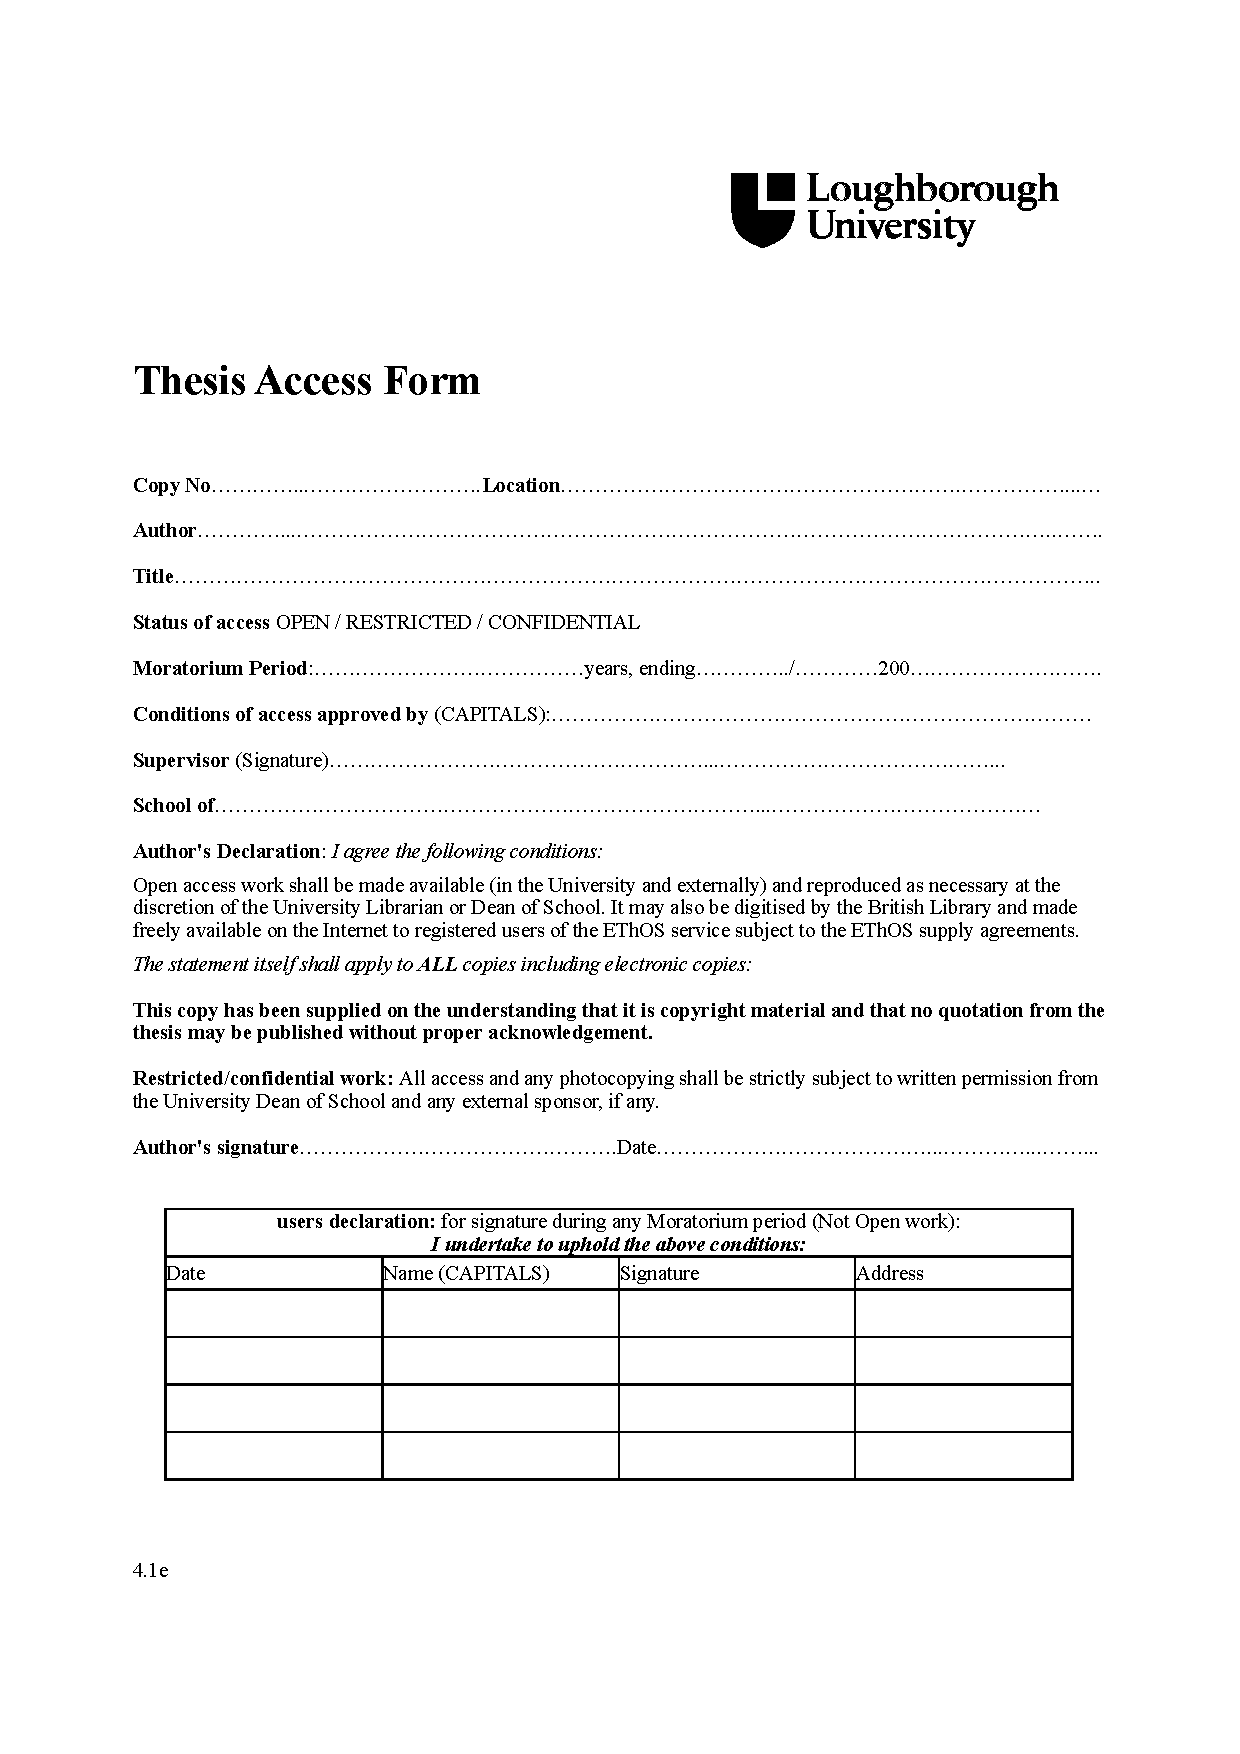
\includepdf[pages=1, pagecommand=, templatesize={5in}{10in}]{Front/LU/access.pdf}
% % Certificate of Originality
% 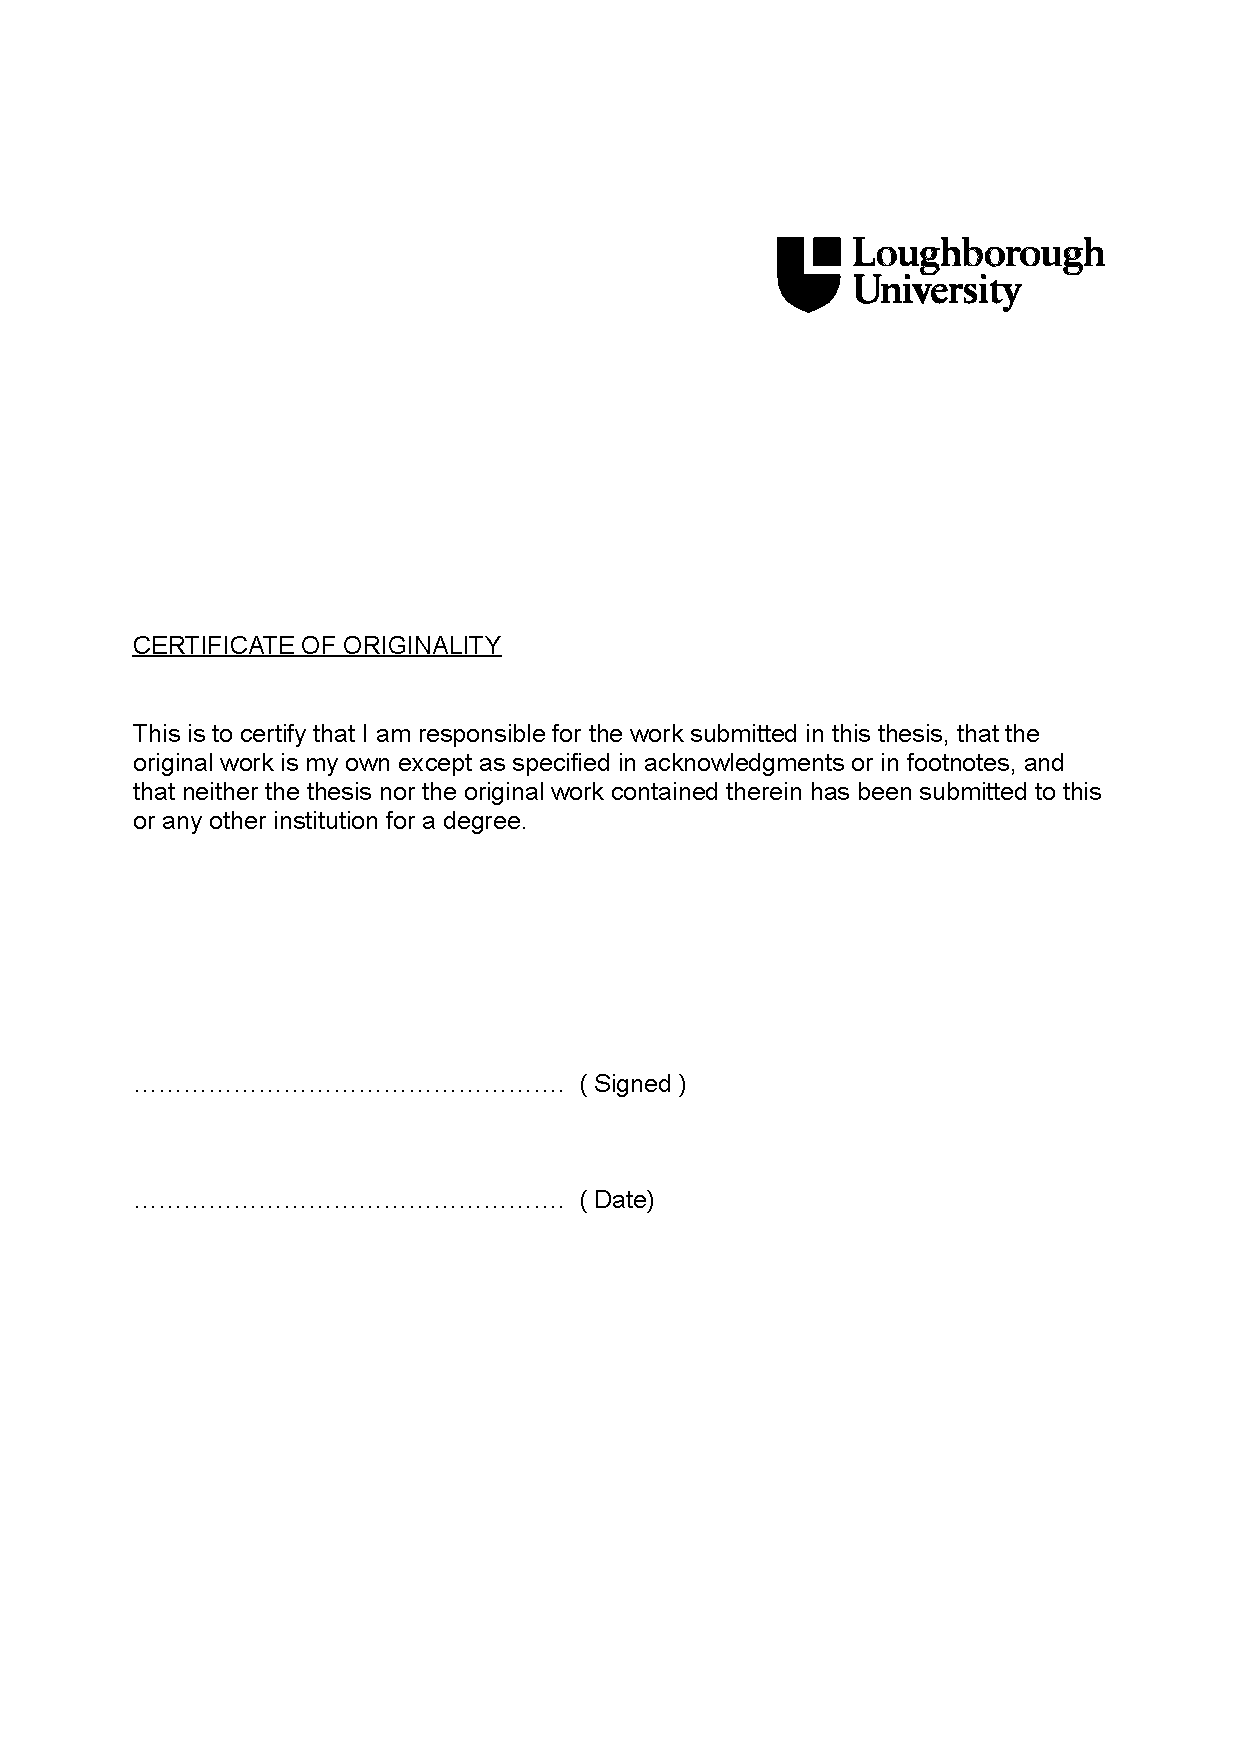
\includepdf[pages=-, pagecommand=, templatesize={5in}{10in}]{Front/LU/origin.pdf}

% Abstract
\addcontentsline{toc}{chapter}{Abstract}
\chapter*{Abstract}
In this coursework, I implement a JPEG Image Compression Simulation using MATLAB as frontend GUI and Python as backend JPEG CODEC. There are 2 simulation parameters $K$ and $Q'$ in the application. 
Several specific design considerations are introduced to the implementation, inclding an end-to-end MATLAB interface, an "Video Compression" functionality and DCT as Matrix Computation.
I conclude that both $K$ and $Q'$ can significantly affect the quality of the compressed image.


% % Acknowledgements
% \addcontentsline{toc}{chapter}{Acknowledgements}
% \chapter*{Acknowledgements}
% Acknowledgement section.

% Set the depth for your table of content
% Currently set at 2 (Chapter, Section, Subsection)
\setcounter{tocdepth}{2}
% Include a table of content
\tableofcontents

% Include a list of figures
\addcontentsline{toc}{chapter}{List of Figures}
\listoffigures

% Include a list of tables
\addcontentsline{toc}{chapter}{List of Tables}
\listoftables

% Include a list of Listings
\addcontentsline{toc}{chapter}{List of Listings}
\renewcommand*{\lstlistlistingname}{List of Listings}
\lstlistoflistings

% Include a list of abbreviations using nomenclature package
%\addcontentsline{toc}{chapter}{List of Abbreviations}
%\printnomenclature[3cm] 

\newpage

% Set page numbering to arabic for body of Thesis
\pagenumbering{arabic}


% To keep everything neat I included each chapter as a separate .tex file
% Each contains a single chapter, they include all the settings defined in this .tex file
% Allows easier moving around of chapters

% Use \include{<path to .tex file>} to include documents
% For example
\chapter{Introduction}
\label{chap:introduction}

This project is based on a mobile robot that has been built with latest AI technology and various sensor capabilities.
It could be programmed in Python.
It has a latest Realsense camera from Intel, which could capture both colour RGB image and depth image and be processed with a Nvidia nano board which supports image processing and deep learning. 
It also has multiple proximity sensors at its front, sides and back.

The task we have done in this project is programming its behaviours and test them to see if it works fully functionally. There are two types of behaviour we have been working on, Reactive Behaviours and Following Behaviours.

\subsection{Reactive Behaviours}
In this part we have designed robot’s behaviour simulate Braitenberg’s vehicle behaviour. 
There are four different behaviours: Love, Fear, Aggression as long as curious. 
We have used a black backpack as our targeted object and used deep learning to train the robot using its camera to recognize that specific backpack in a complex environment. 
When the robot has detected the targeted object, it will initiate the behaviour that we have been assigned.

\subsection{Following Behaviours}
In this part we programmed the robot to follow a human that has been detected by its RGBD camera and not only follow its movement, but also keep a safe distance from targeted human. 

For each behaviour, aspects of assumptions, system design, implementation and test \& analysis are described in details.






\chapter{Robot Configuration}
\label{chap:configuration}

\chapter{Reactive Behaviours}
\label{chap:reactive}

We are going to design a robot which could do multiple Braitenberg’s behaviours, which has four specific behaviour, they are love, aggression, fear and curious. 
Firstly, finding a good targeted object is very important. It needs to be easy to recognize while robot is swing on the floor. 
By several testing we have decided that a backpack is the best static targeted object to use in labs. Because it not only contains different unique features, but also the size of the object is suitable for camera to recognize. 
Before it starts doing behaviour, it needs to wonder around to find targeted objects. 
Once it has targeted objected in its bounding box, it starts the behaviour that we designate. 
For each unique behaviour, we need to consider circumstances for each one of them.

\section{Assumptions}

Several assumptions are made in our design of reactive behaviours.

\begin{enumerate}
    \item There is no obstacle between the object and the robot.
    \item There is only one object of interest in the environment.
\end{enumerate}


\section{System Design}

\subsection{Flow Chart}

The algorithm of reactive behaviour is shown in Figure \ref{fig:reactive}. After we initiate the robot, the robot will rotate itself to scan around the area until it finds the targeted object.  While RGBD camera successfully lock the object, it will put a blue bounding box at it, then it will further process the image that it has been read to make sure it is the real targeted object, at that time, bounding box will become red and it will process what behaviour task we have been given in our computer. 
After one behaviour has been finished, it will start the previous process again and wait for command.

\begin{figure}
\centering
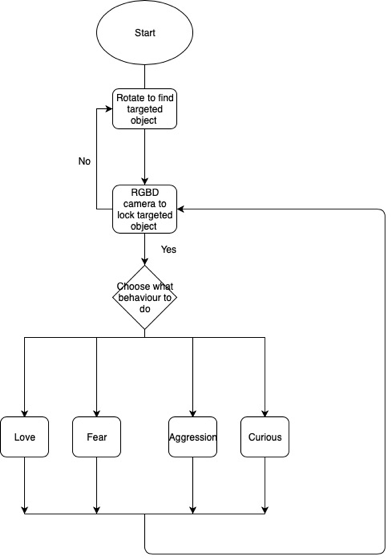
\includegraphics[width=0.5\textwidth]{reactive}
\caption{Flow Chart of the Mobile Robot with Reactive Behaviours.}
\label{fig:reactive}
\end{figure}

\subsection{Aggressive Behaviour}

Aggression means feelings of anger or antipathy resulting in hostile or violent behaviour; readiness to attack or confront in English, so we want robot to react some critical movements after it successfully located target. A significant accelerate of speed will be the key point of aggressive behaviour. It also should be stop from a safe distance to avoid collision. So, Depth sensor function in camera will be useful in this circumstance.

\begin{figure}
\centering
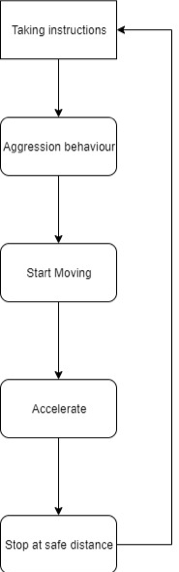
\includegraphics[width=0.3\textwidth]{aggressive}
\caption{Aggressive Behaviour.}
\label{fig:aggressive}
\end{figure}

Figure \ref{fig:aggressive} describes Aggressive Behaviour in details.
For Aggressive Behaviour, after robot taking instructions, it will initiate its motor to a stable speed, while depth camera has a reading that targeted object has beyond safe distance, it will centralise its direction towards object, then it will accelerate significantly towards targeted object. While depth camera has reading that it reached safe distance, the motor will stop to avoid collision to the target.

\subsection{Fear Behaviour}

In opposite to Aggression, fear behaviour should keep a distance from the target. So RGBD camera should be use as well. While robot has detected the targeted object, it firstly using depth camera to read distance between object and itself, then it will move backward in a significant speed. The speed should also decrease as the distance between targeted object increase.

\begin{figure}
\centering
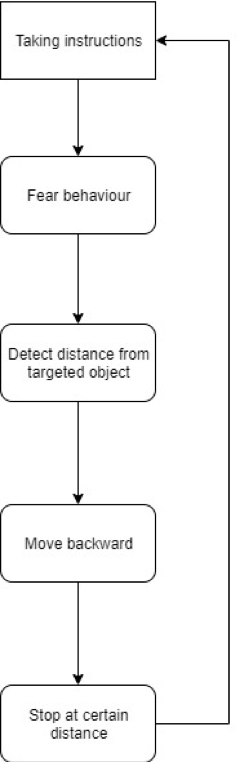
\includegraphics[width=0.3\textwidth]{fear}
\caption{Fear Behaviour.}
\label{fig:fear}
\end{figure}

Figure \ref{fig:fear} describes Fear Behaviour in details.
In contrast to Aggressive Behaviour, Fear is doing opposite movement, it also starts by wondering around. While targeted object has been detected and confirmed, it will quickly move backwards from the target. There is also a deceleration of speed that we have designed at this part, which means the farther away the robot is from the targeted object, the slower it moves.

\subsection{Curious Behaviour}

Curious means eager to know or learn something, as a robot with only movement physical function, we define curious as a movement that contains moving forward and moving backward constantly. While targeted object is detected in camera’s sight, it will seek if the target is at left side or right side, then it will move left forward or right forward correspondingly.

\begin{figure}
\centering
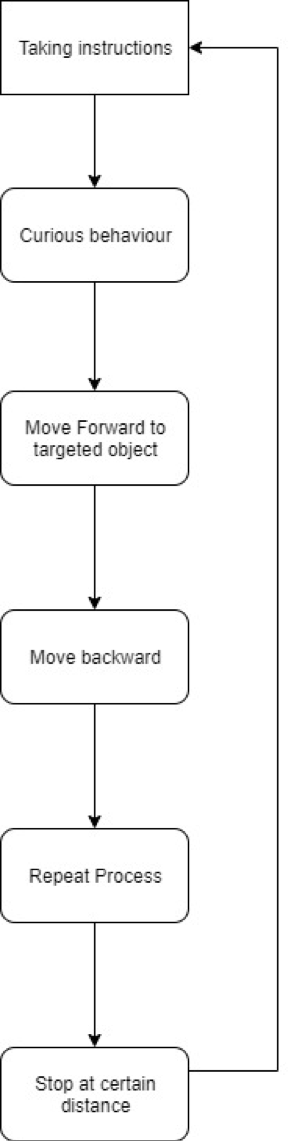
\includegraphics[width=0.3\textwidth]{curious}
\caption{Curious Behaviour.}
\label{fig:curious}
\end{figure}

Figure \ref{fig:curious} describes Curious Behaviour in details.
Curious Behaviour uses same direction recognition technique as ‘Love’ behaviour, by defining what location of targeted object that robot is facing; For example If targeted object is on left side of the robot, robot will move left forward towards the target, while it getting closer, it will moving backward, and moving towards the target again until it reaches the safe distance.

\subsection{Love Behaviour}

Love is hard to define for a simple physical movement robot since it’s an emotional vocabulary. We defined love as move slowly and shake its head while moving. When targeted object has been detected, it will turn left, then go forward a bit, then move right, forward a bit. It terminates the movement after reaching the safe distance from object.

\begin{figure}
\centering
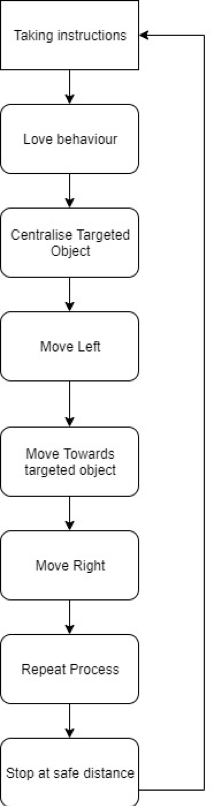
\includegraphics[width=0.3\textwidth]{love}
\caption{Love Behaviour.}
\label{fig:love}
\end{figure}

Figure \ref{fig:love} describes Love Behaviour in details.
When t robot is taking instructions of doing ‘Love’ behaviour, it will firstly find targeted object, after successfully put the bounding box on the targeted object, it will define whether object is on its left or on its right, then it will turn its direction to the opposite, then it will move forward a bit and turn its direction again, to do this movement is simply because wants robot to combine this series of movement, after-all the robot will shakes its head as he walks towards the target.

\section{Implementation}
Task 1 was to implement the Braitenberg behaviours which are love, fear, aggression and curiosity. 
Each of the behaviours the robot needs to first find the target we have specified. This is done within the process function which first calculates all the detected objects in the view of the camera. 

\begin{lstlisting}[language=Python]
detections = model(imgsized)
\end{lstlisting}

We then filter out the detections found to give us an array of only objects that we are interested in. 

\begin{lstlisting}[language=Python]
matching_detections = [d for d in detections[0] if d['label'] == int(label_widget.value)]
\end{lstlisting}

Finally, each detection has a confidence field which is used to show the confidence (0-1) that the object is the one we want. If the confidence is less than 0 (i.e. not our object) we draw a blue bounding box around it otherwise if the object is what we want, we draw a red bounding box around it. 

Additionally, we keep a count of the number of objects that the camera sees so we have a counter of all the objects on the left-hand side of the screen, centre of the screen and right-hand side of the screen. 

This is done with the following code:
\begin{lstlisting}[language=Python]
if (bbox[0]+bbox[2])/2 < 2/5.0:
                left_count = left_count + 1
            elif (bbox[0]+bbox[2])/2 > 3/5.0:
                right_count = right_count + 1
            else:
                center_count = center_count + 1
\end{lstlisting}

When the robot does not find the object we want, the robot does a 360 rotation (starting left or right depending on how many objects there are on that side, so if there are more objects on the right hand side, the robot will start turning  towards the right). Once the object has been detected, the emotion that has been selected will be executed.

A dropdown widget has been added to allow users to specify the behavior they want. By default this is set to love.

\subsection{Aggressive Behaviour}
The aggression behavior is implemented by first having the robot move towards the side of the screen that has the most objects. Once the target object has been located, the robot will move towards the object increasing its speed the closer it gets to the object. Once the robot has reached a distance of 1200 or less, the robot stops. The gradual speed up from slow to fast going to the object is how we have implemented aggression. 

The code for agression: 
   
\begin{lstlisting}[language=Python]
    if distance < 1200:
        robot.stop()
    elif left_count > right_count and left_count > center_count:
        robot.forward_left(max((5000-distance)/2500*2+0.3, 0.3))
    elif right_count > left_count and right_count > center_count:
        robot.forward_right(max((5000-distance)/2500*2+0.3, 0.3))
    else:
        robot.forward(max((2000-distance)/2000*2, 0.3))
\end{lstlisting}

The code shows how the robot stops if too close and how it moves left, right or center depending on what side of the screen the object is on. The speed is increased as the distance is shortened. 


\subsection{Fear Behaviour}
Fear is implemented by first havimg the robot robot move in the direction where there are the most objects (left, centre or right) then once it detects the target object and is less than 2500mm in distance, the robot goes backwards in reverse quckly. The robot can be observed to slow down the further away it is from the object. 

This is done with the following code:

\begin{lstlisting}[language=Python]
            if distance < 2500:
                robot.backward(max((3000-distance)/3000*2, 0.3))
\end{lstlisting}

We choose that 3000 is the max distance we can do this from and that the speed can range between 0-1. Thus this gives the affect of fear with the control of speed.


\subsection{Curious Behaviour}
For curiosity we have made the robot go towards the area that has the most amount of objects. This is because we believe that where there are more objects, the robot is more curious. The robot will stop if the distance between the object is less than 800mm otherwise it will either go left, right, or center depending on object count on that side. The code to see the behavior is in the curious function were a direction is specified and the movement happens accordingly. For the curious behavior we have made the robot go forward and backwards towards the target object once it has been located. 

\subsection{Love Behaviour}
The way love is implemented is once the robot has found the target object, the robot moves left, moves forward, moves right and then moves forward again. This results in the robot moving in a sort of short ziggzag fashion towards the object. This can be observed in the love function. Additionally, to keep the robot on track towards the object, in the process function we check if the distance is bigger than 100mm and depending on what side of the screen the most amount of objects are, we turn the robot towards that direction (i.e. if there are more objects on the left, we make the robot turn left). Once the robot reaches a safe distance of 900mm the robot stops. 

The love function:
\begin{lstlisting}[language=Python]
    def love():
        global love_flag
        if love_flag == 0:
            robot.left(0.5)
        elif love_flag == 1:
            robot.forward(0.3)
        elif love_flag == 2:
            robot.right(0.5)
        elif love_flag == 3:
            robot.forward(0.3);
        love_flag = (love_flag + 1) % 4
\end{lstlisting}

The love\_flag is used to keep track of the movement that had been performed. This is so that we can control the movement of the robot in stages.

\section{Test \& Analysis}

Our group test the task 1 in the computer master students Lab. In this Lab, we put the robots on the carpet. Because there are too many chairs and people. So, we decide to use the cup first. But is too small to recognize. Then we test the keyboard, but it still hard for robot’s camera to recognize. Finally, we decide to use the black bag as the object. Because it is big enough to be easy to recognize.


\subsection{Aggressive Behaviour}

When we test this function, after choosing the aggressive. The robot will approach target slowly. When it close to the object, the robot will accelerate significantly. In order not to damage the robot, we design to stop in front of the target. Instead of going randomly, we design the if the robot cannot find the object. The robot will rotate in place, until find the object.

\begin{figure}
\centering
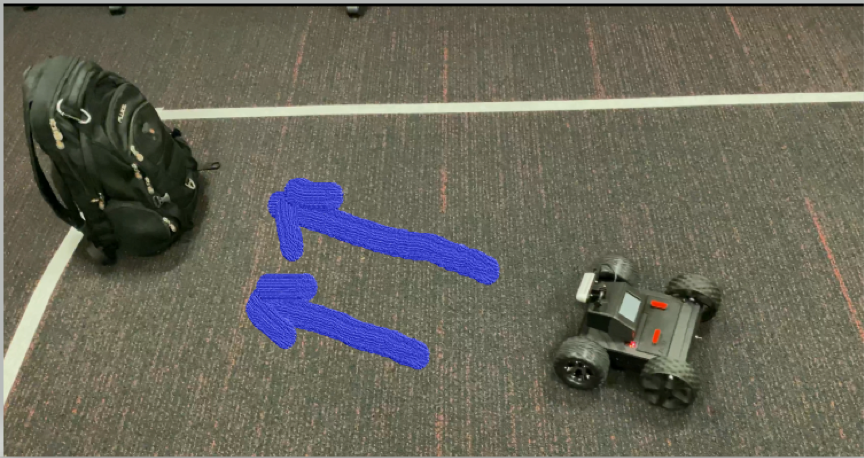
\includegraphics[width=0.8\textwidth]{aggressive-test}
\caption{Testing of Aggressive Behaviour.}
\label{fig:aggressive-test}
\end{figure}

From the capture in the video shown in Figure \ref{fig:aggressive-test}, we can find that the process of accelerate is very clearly. It can show this function is accomplished perfectly. During the test, we found that the need some distance to show this function obviously. 

\subsection{Fear Behaviour}

When we test this function, after choosing the fear. The robot will leave the object quickly. Just like the real fear. At first, we set the stop distance as 2500. During the test, the 2500 is too far away sometimes the camera will lose the object because the distance is too big, then the robot will rotate in place to find the object again. In order to this situation. We change the distance as 1800. 

\begin{figure}
\centering
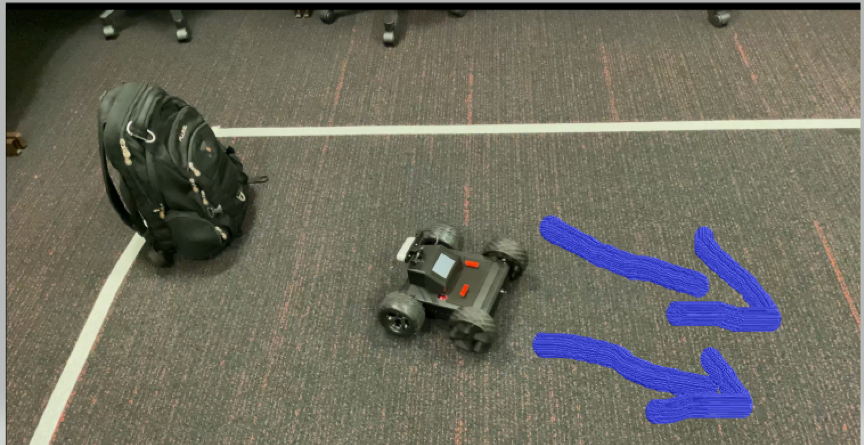
\includegraphics[width=0.8\textwidth]{fear-test}
\caption{Testing of Fear Behaviour.}
\label{fig:fear-test}
\end{figure}

From the capture in the video shown in Figure \ref{fig:fear-test}, we can find that the distance 1800 is pretty appropriate for the test. The leave process is obvious. The function is completely accomplished.

\subsection{Curious Behaviour}

When we test this function, after choosing the curious. The robot will find where is the object, then forward and backward during the forward process. There are some questions when we test this function. At first, we set the forward or backward speed to high. Then the camera also easy to lose the object. So, we turn down the speed. After that, the result is better than before.

\begin{figure}
\centering
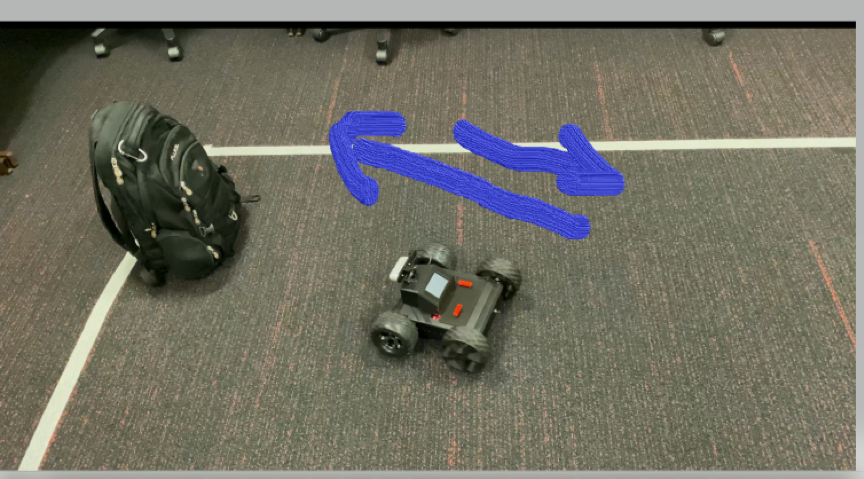
\includegraphics[width=0.8\textwidth]{curious-test}
\caption{Testing of Curious Behaviour.}
\label{fig:curious-test}
\end{figure}

From the capture in the video shown in Figure \ref{fig:curious-test}, the robot forward and backward and during this process, the camera still can get the object. So, this function is successful.


\subsection{Love Behaviour}


When we test this function, after choosing the love. The robot will find where is the object, then turn left and turn right, like shake the robot. During the test we find some question, the robot is hard to find the project during turn left and right. It is easy to lose the object when the process of making a turn. At first, we segment the frame to 3 part, left, right and center. Then we found it is easy to lose the object. So, we change the frame and segment it to 5 part. The left two parts as left. The middle part as the center. And the right two parts as the right. The robot turns left or turn right by in bounding box which part contain the most objects. After do this, the robot is better to find the object during the turning process.

\begin{figure}
\centering
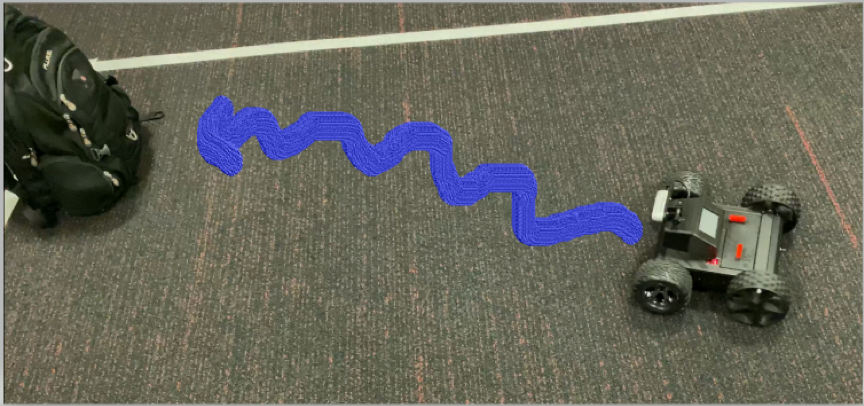
\includegraphics[width=0.8\textwidth]{love-test}
\caption{Testing of Love Behaviour.}
\label{fig:love-test}
\end{figure}

From the capture in the video shown in Figure \ref{fig:love-test}, we can find that the camera can recognize the object from beginning to the end. And perfectly complete the love function turn left and turn right during the forward process.

\subsection{Facing Backward to the Object}

In order to test the stability of the function. We also test some special situation not test before. For example, the robot is facing back to the object, side to the object and no object at all.

\begin{figure}
\centering
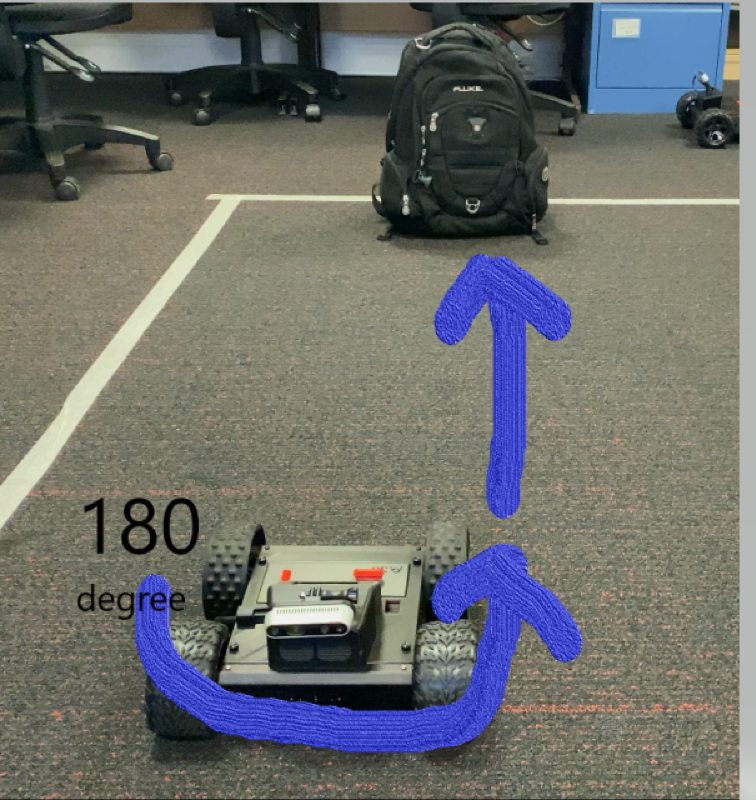
\includegraphics[width=0.8\textwidth]{back-test}
\caption{Testing of Facing Backward to the Object.}
\label{fig:back-test}
\end{figure}


In this situation, we put the black bag in the back of the robot, the robot will make a turn in place for about 180 degrees angle to find the object in the back of the robot. After find the object, the expected outcome is the same with the actual outcome. The robot can find the object quickly.

Just like the capture in the video shown in Figure \ref{fig:back-test}, we can find it can find the object in the back of the robot.

\subsection{Facing Sideways to the Object}

In this situation, we put the black bag in the side of the robot, the robot will make a turn in place for about 90degree angle to find the object in the side of the robot.

\begin{figure}
\centering
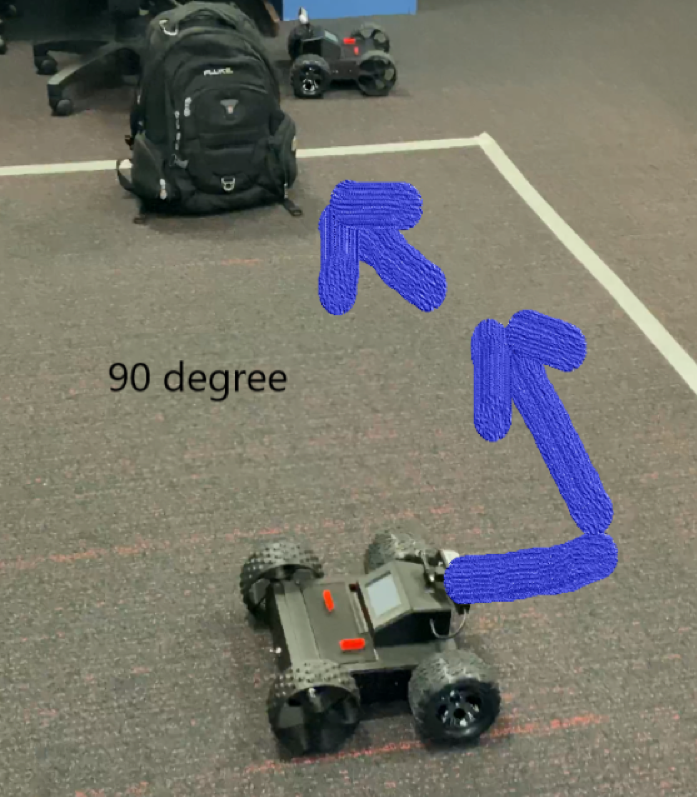
\includegraphics[width=0.8\textwidth]{side-test}
\caption{Testing of Facing Sideways to the Object.}
\label{fig:side-test}
\end{figure}

From this capture shown in Figure \ref{fig:side-test} we can find the robot can find the object in the side of the robot.

\subsection{No Object in the Environment}
In this situation, we do not put anything around the robot.

\begin{figure}
\centering
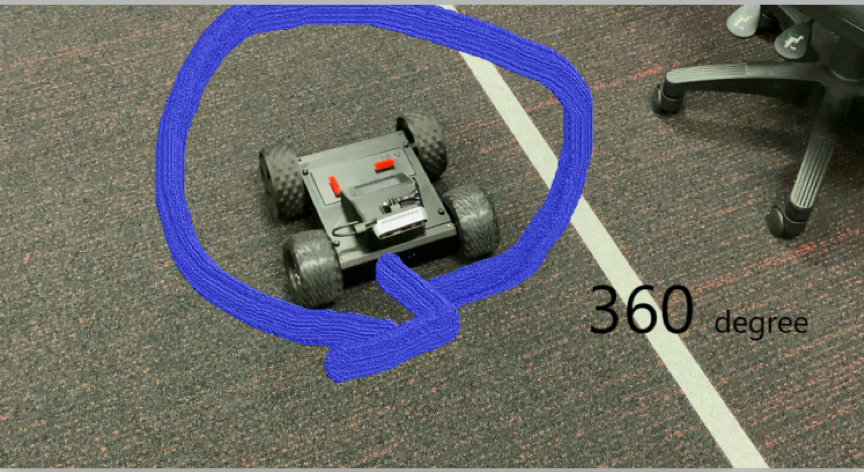
\includegraphics[width=0.8\textwidth]{no-test}
\caption{Testing of No Object in the Environment.}
\label{fig:no-test}
\end{figure}
 
From this capture shown in Figure \ref{fig:no-test}, we can find the outcome the robot is turning in place for 360 degrees again and again.

\chapter{Following Behaviours}
\label{chap:following}

In this chapter, we describe the design, implementation and testing of a mobile robot with following behaviours.
The mobile robot follows a designated person, while keeping a safe distance.
When the designate person is not on the scene, the robot should wander around to look for the person.

\section{Assumptions}

Several assumptions are made in our design of following behaviours.

\begin{enumerate}
    \item There is no obstacle between the person and the robot.
    \item When more than one person are on the scene, the robot is given instruction on which person to follow. That is, a person is designated to be followed.
    \item The designated person is dressed differently to other persons on the scene such that the robot can tell the difference.
\end{enumerate}

\section{System Design}

\subsection{Flow Chart}

A flow chart of the mobile robot is shown in Figure \ref{fig:following}.
When the robot starts and receives the first image from the camera, it locates all persons on the image using an object detection model \citep{howard2017mobilenets,liu2016ssd}.
If no person is found from the camera image, the robot activates "Wander Behaviour."
If one or more persons are located, for each person located, a bounding box and a confidence score are given by the model.

Each bounding box is resized and compared against the target image for a similarity score using the euclidean distance.
The person with the highest similarity score is selected.
During the comparing stage, the user may also change the target image to any bounding box of located person.
By default, the target image is a blank image.

If the highest similarity score is lower than $0.7$, "Wandering Behaviour" is activated.
Otherwise, both "Collision Avoidance Behaviour" and "Person Following Behaviour" are activated. However, the output action from "Collision Avoidance Behaviour" has higher priority than "Person Following Behaviour".

Once the robot finishes the action and receives a new update from the camera, it will repeat from locating all persons on the scene again.

\begin{figure}
\centering
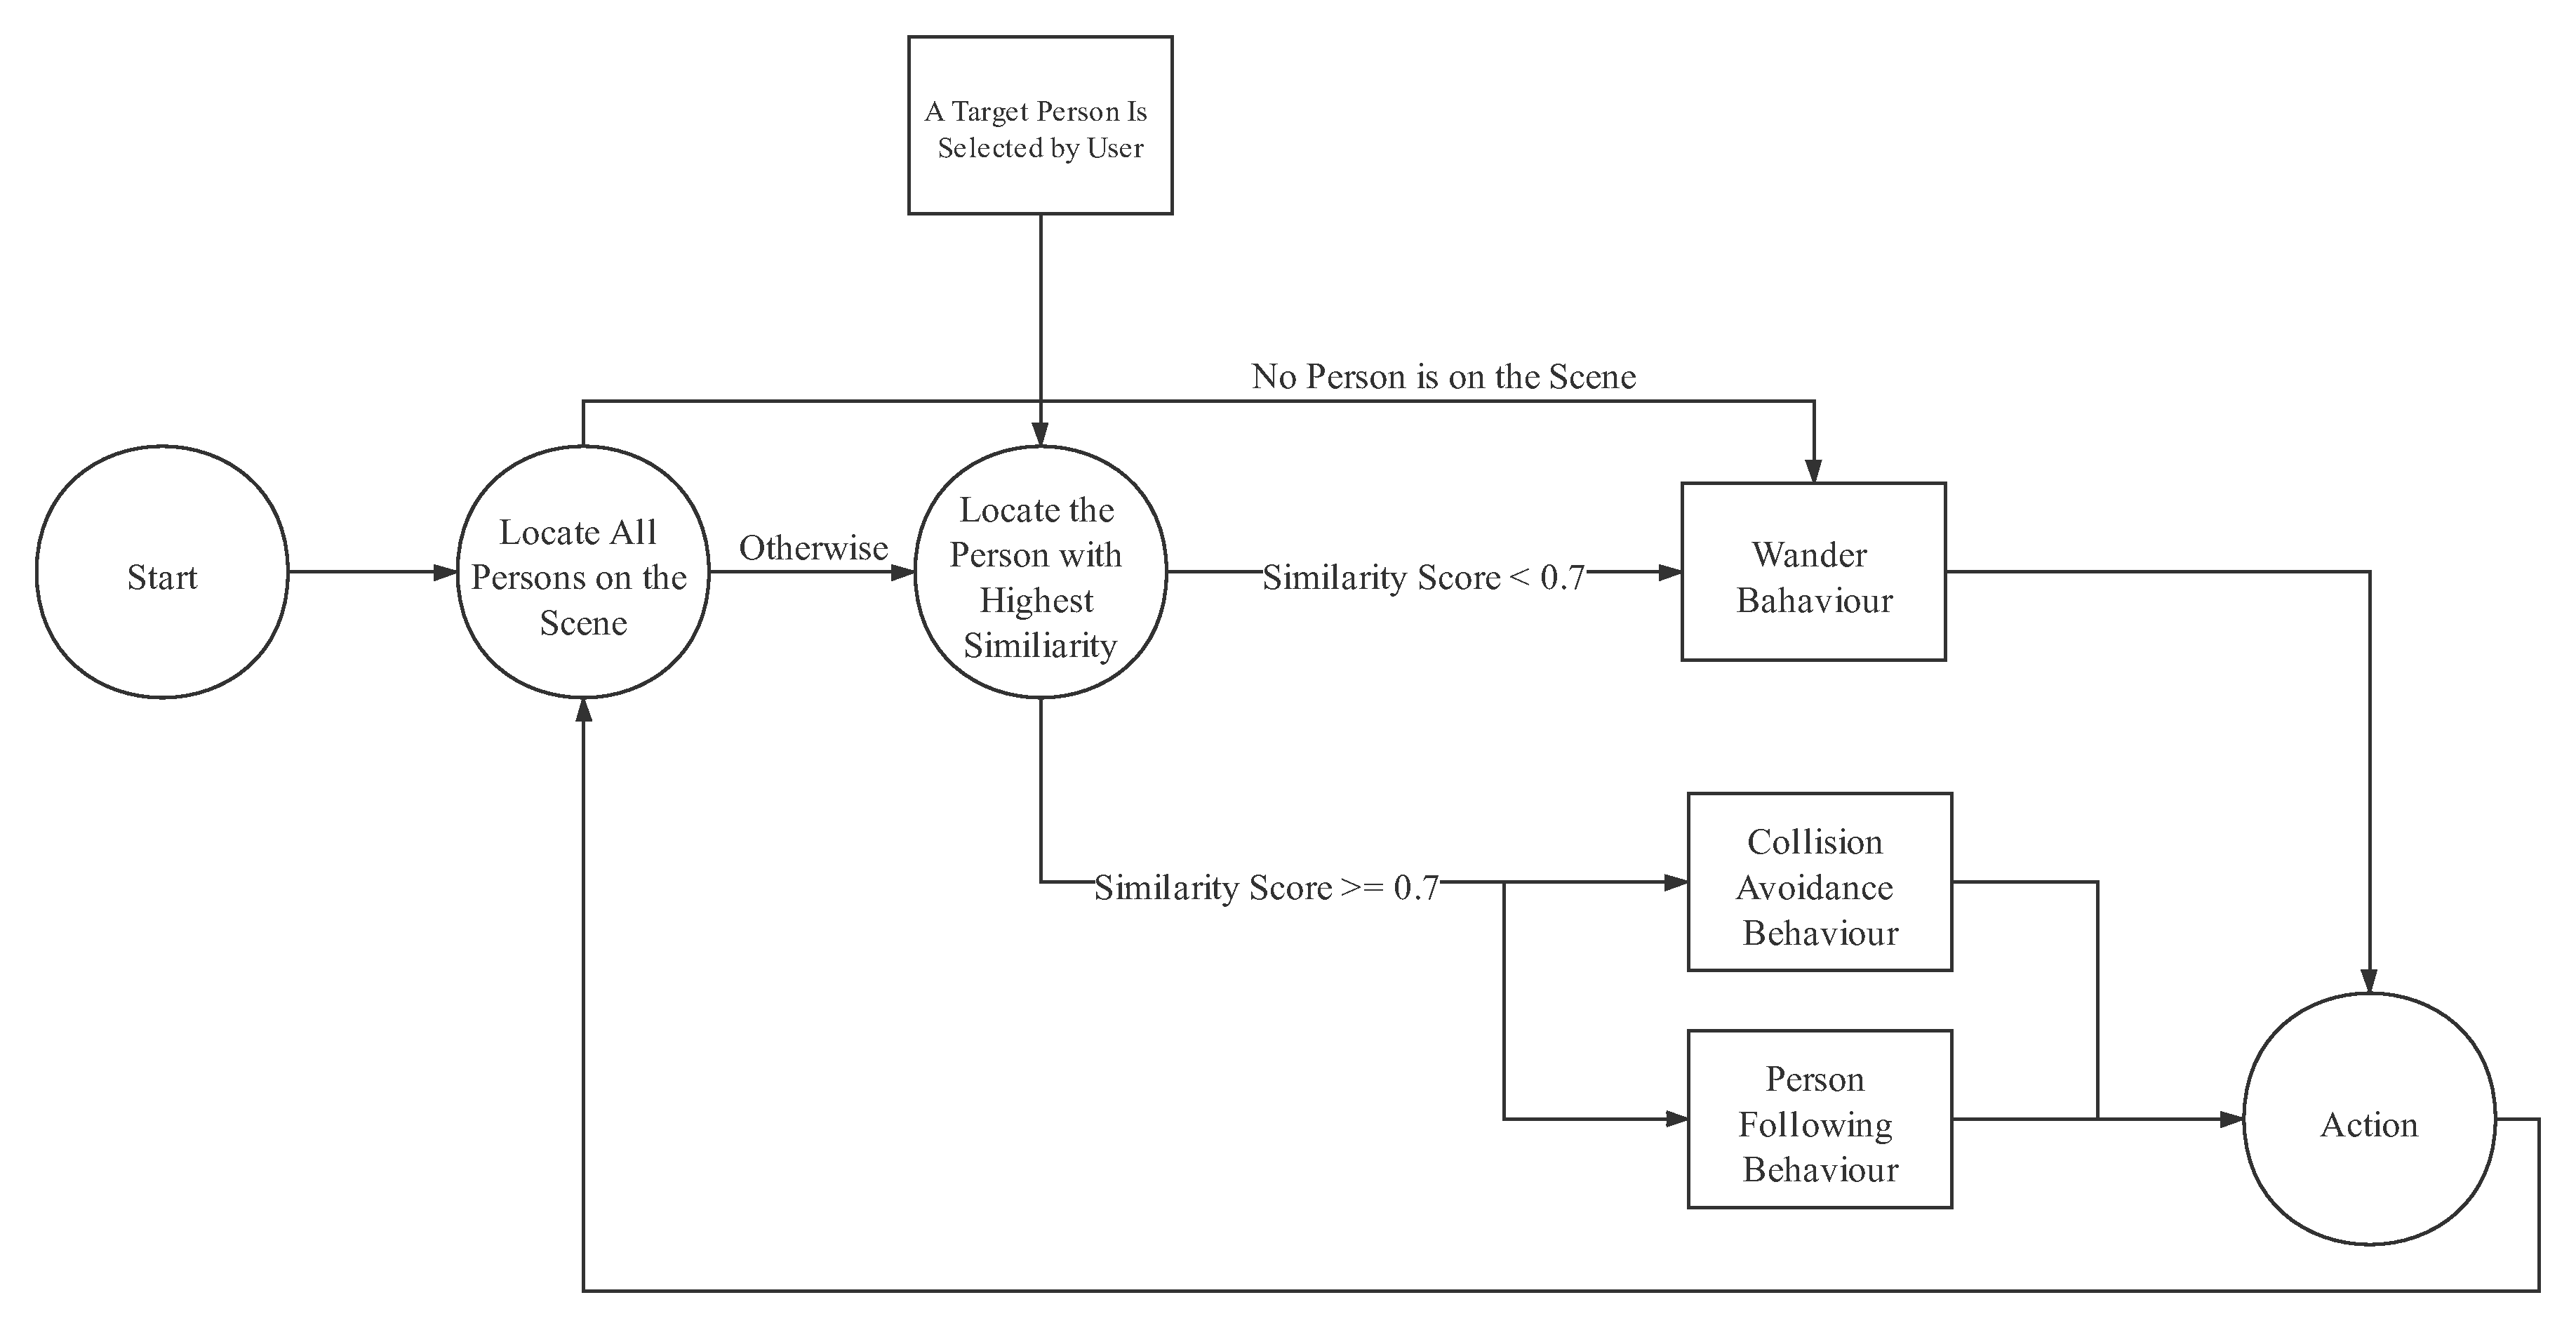
\includegraphics{following}
\caption{Flow Chart of the Mobile Robot with Following Behaviours.}
\label{fig:following}
\end{figure}

\subsection{Wandering}
Our initial design of Wandering behaviour is to keep moving forward and turn left when an obstacle is found in front of the robot.
However, we observe that such behaviour leads to frequent dead ends and bumping due to the size of the robot and the complexity of our environment.
The initial Wandering Behaviour is replaced with self-rotating as shown in Figure \ref{fig:wander}.
That way, the robot will keep rotating in the same direction until a person is located.
It will not move into the dead end or bump into the obstacle.

\begin{figure}
\centering
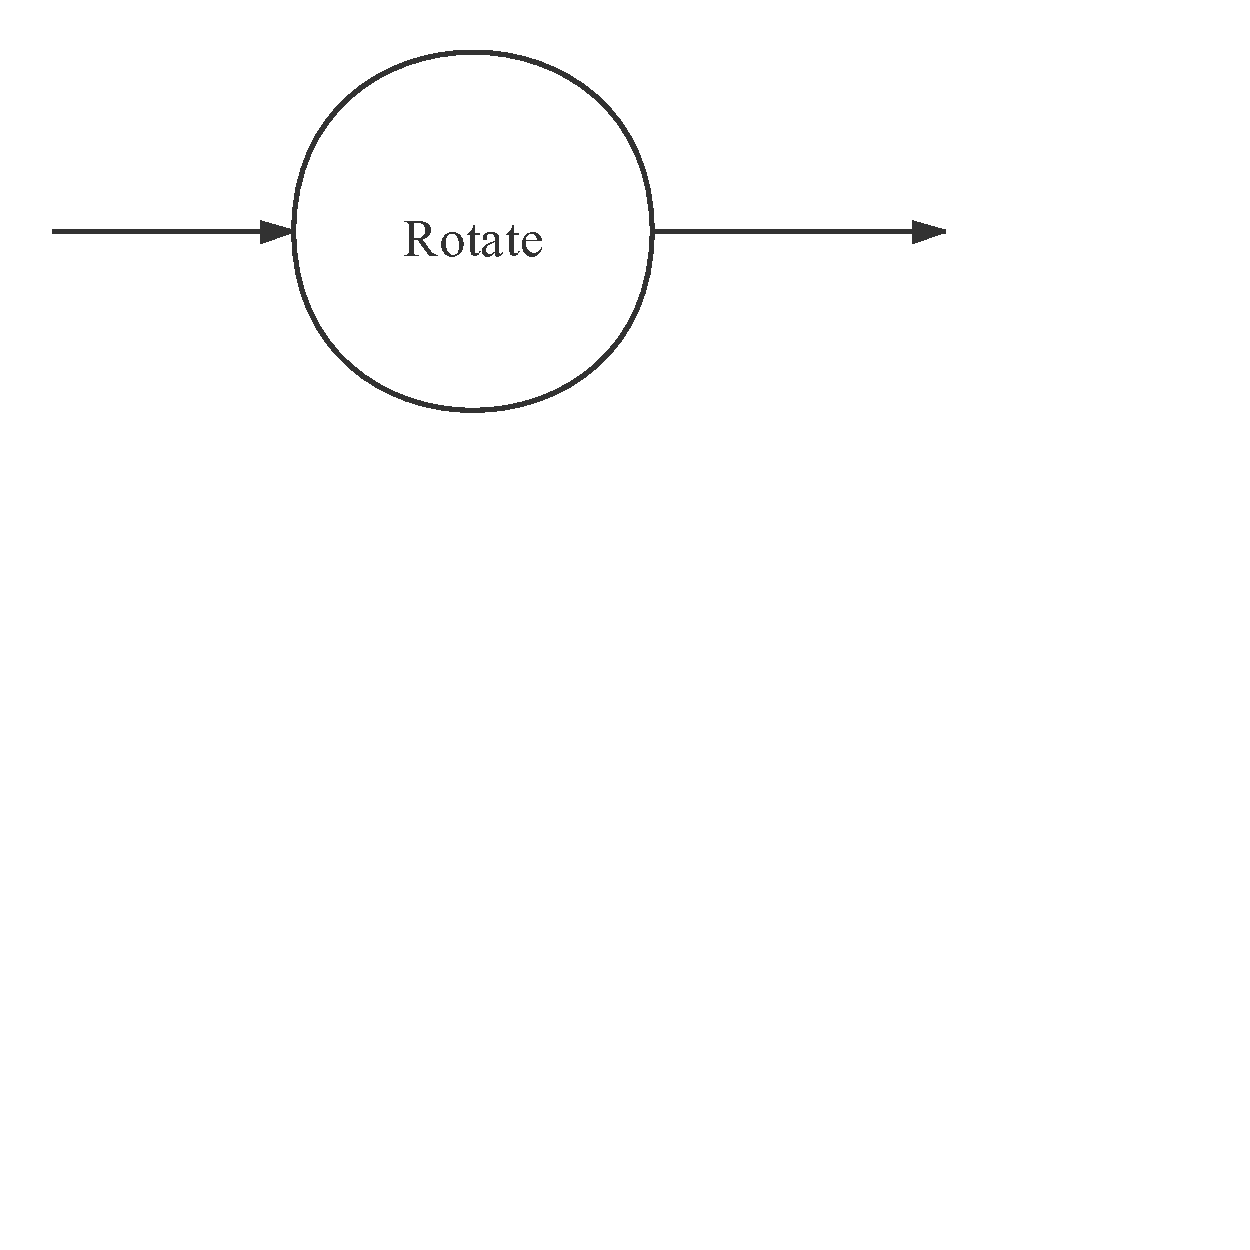
\includegraphics[width=0.5\textwidth]{wander}
\caption{Wandering Behaviour of the Mobile Robot.}
\label{fig:wander}
\end{figure}



\subsection{Collision Avoidance}
Collision Avoidance Behaviour prevents robot from bumping into the designated person and always has higher priority than Person Following Behaviour.
Figure \ref{fig:collision} describes the behaviour in details. The distance between the robot and the designated person is computed using the camera's depth information.
If the distance is smaller than $300$ mm, the robot moves backward to avoid bumping into the person.
If the distance is equal or larger than $300$ mm and smaller than $600$ mm, the robot stops moving.
Therefore, the robot always keeps a safe distance between $300$ and $600$ mm from the person when it stops moving.

\begin{figure}
\centering
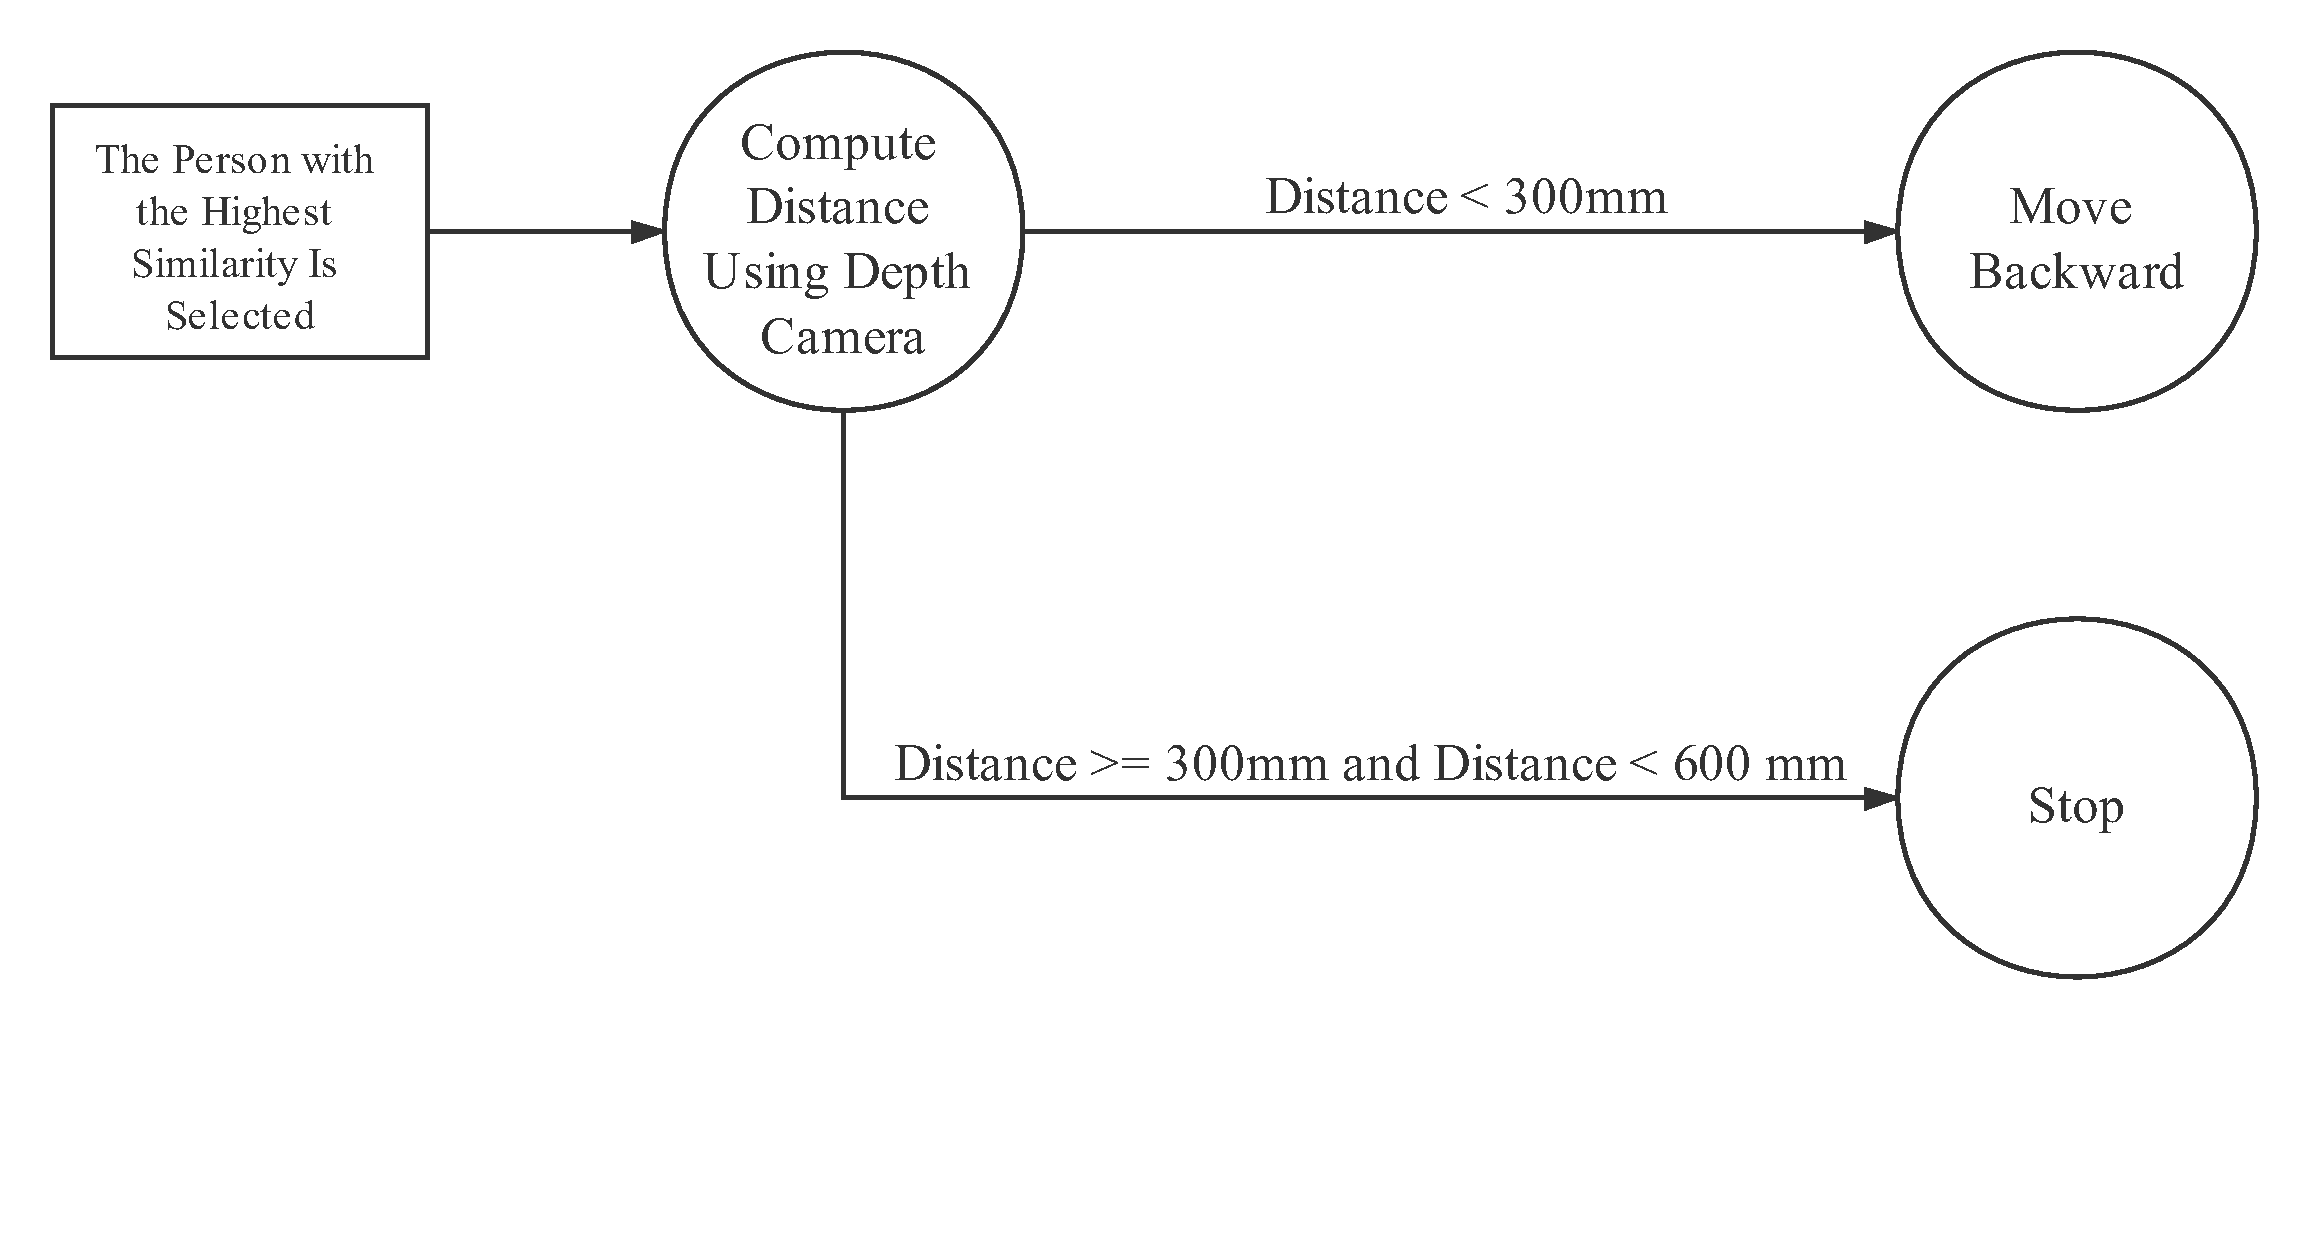
\includegraphics[width=\textwidth]{collision}
\caption{Collision Avoidance Behaviour of the Mobile Robot.}
\label{fig:collision}
\end{figure}

\subsection{Person Following}
Person Following Behaviour keeps tracking the designated person and moving the robot to the person.
Figure \ref{fig:person} describes the behaviour in details.
The target image is first replaced with the new bounding box if the similarity between them is larger then $0.9$.
This action keeps the robot updated with the information of the target. It prevents the robot from decreasing similarity score over time and losing the target in the end.

The center of the bounding box in x-axis is later computed to determine whether the person is on the left, center or right.
If the person is on the left side, the robot rotates to the left and vice versa.
If the person is in the center area, the robot moves forward.


\begin{figure}
\centering
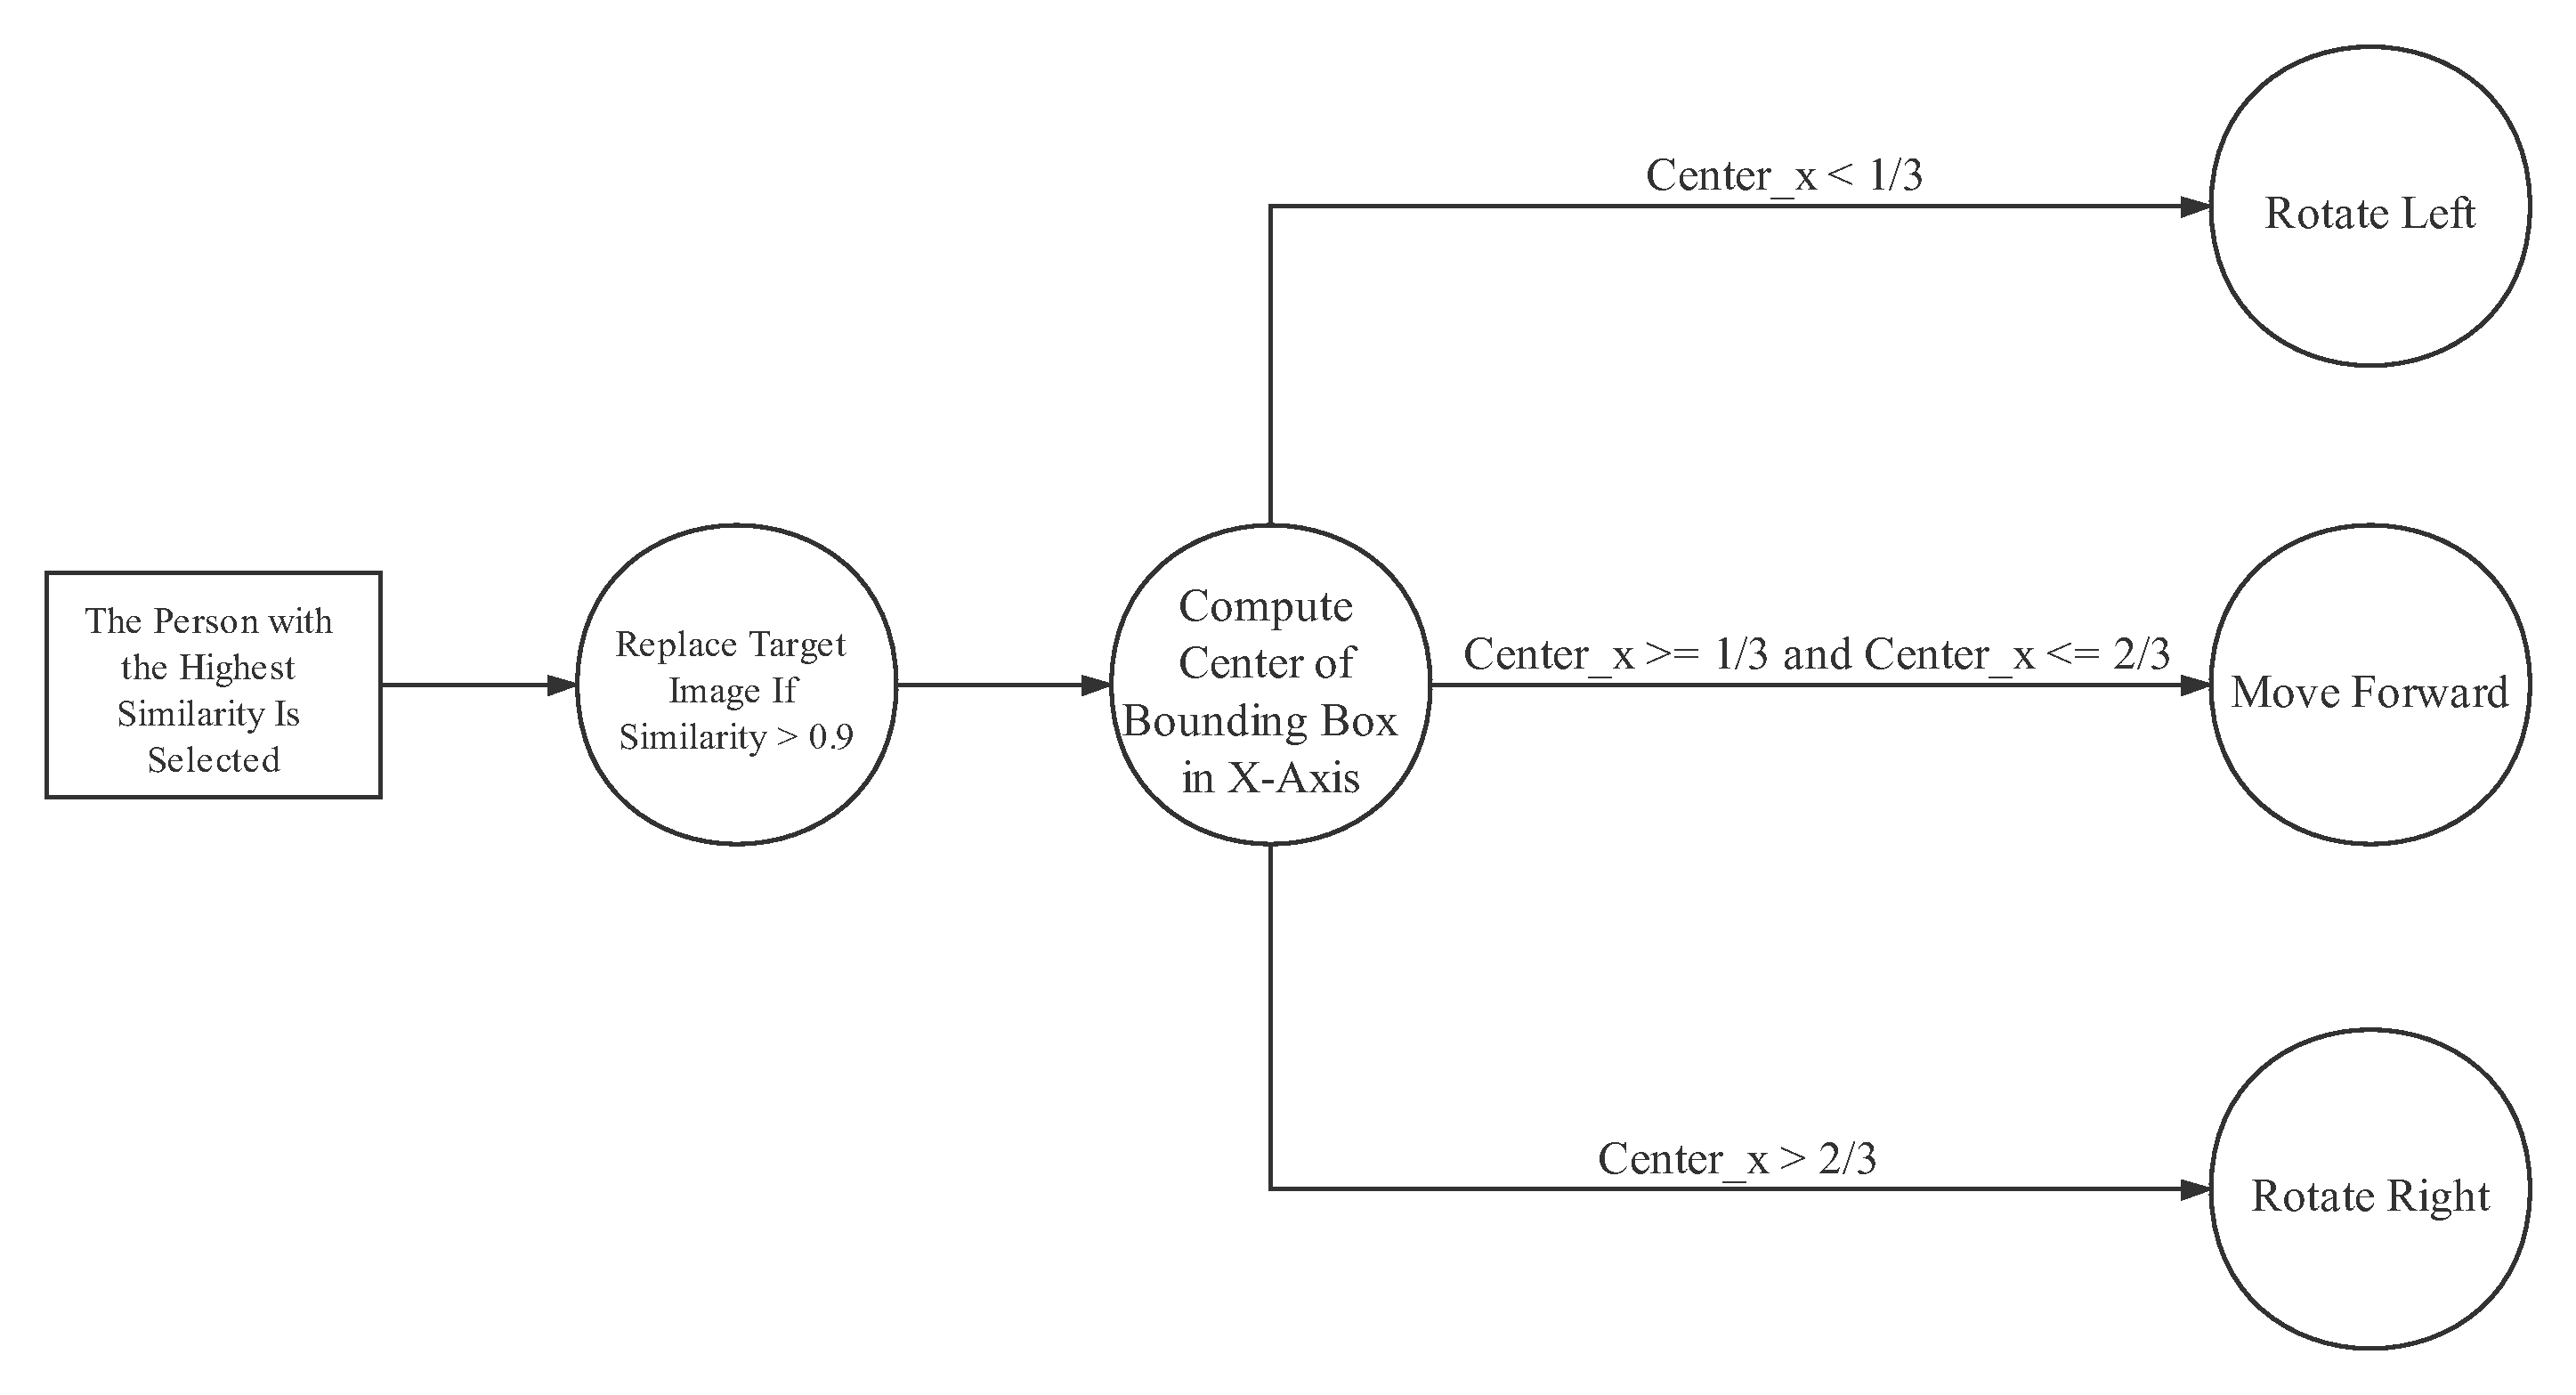
\includegraphics[width=\textwidth]{person}
\caption{Person Following Behaviour of the Mobile Robot.}
\label{fig:person}
\end{figure}

\section{Implementation}
The following behaviours are implemented in Python Programming Language and Jupyter Notebook environment.
The implementation uses the source code from Tutorial 5 as the framework and improves upon that.
Several important adjustments are made and described as follows.

\subsection{Computing Similarity Scores}
After all persons on the scene are located using a object detection model, a similarity score between bounding box of each person (variable named \texttt{obj}) and the target image (variable named \texttt{target}) is computed.
Both \texttt{obj} and \texttt{target} are resized to a resolution of 300-by-300 using \texttt{cv2.resize} function.
Both \texttt{obj} and \texttt{target} are converted to HSV color space using \texttt{cv2.cvtColor} function and later normalised through being divided by $255$.
The similarity score between \texttt{obj} and \texttt{target} is defined $1 - distance_{euclidean}(obj, target)$.

\subsection{Computing Distance}
In Collision Avoidance Behaviour, the distance between the designated person and the robot is computed.
Applying the bounding box of the person to the depth image, a matrix of depths inside the bounding area is retrieved.
The distance between the person and the robot is simply the minimum non-zero value in the matrix.

\section{Test \& Analysis}
Two testing scenarios are performed and analyzed in this section.

\subsection{Single Person Following}
In this scenario, only one person is presented in the environment.
The robot is expected to follow the person around the room.

Figure \ref{fig:follow-test} shows an video capture of our testing scenario.
As the person walks around in the room, the robot keeps following in a safe distance and never loses track of the person.

\begin{figure}
\centering
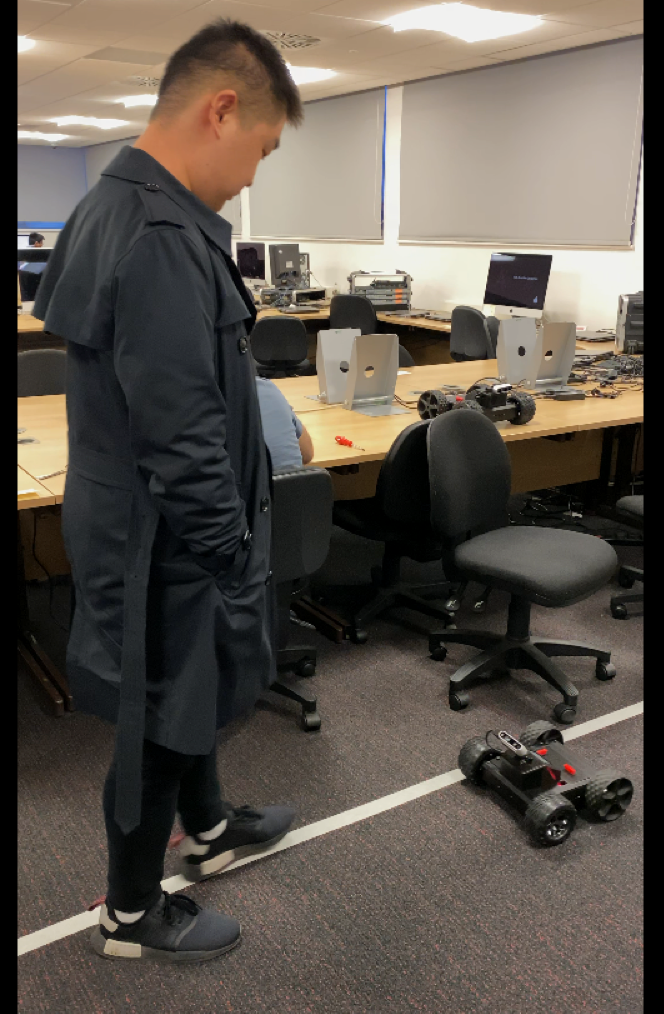
\includegraphics[width=0.8\textwidth]{follow-test}
\caption{Testing of Single Person Following.}
\label{fig:follow-test}
\end{figure}

\subsection{Single Person Following under Attempted Hijacking}
In this scenario, two persons are presented in the environment. One person is chosen as the designated person to follow.
The other person makes several attempts to hijack the robot by stepping in front of the designated person and then walking away.
The robot is expected to always follow the designated person and not follow the other person.

\begin{figure}
\centering
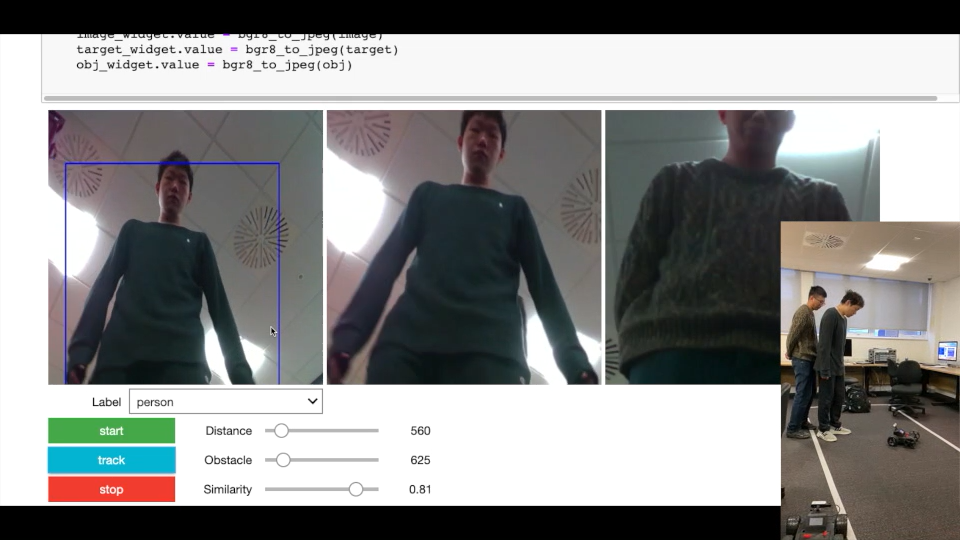
\includegraphics[width=0.8\textwidth]{follow-test-hijack}
\caption{Testing of Single Person Following under Attempted Hijacking.}
\label{fig:follow-test-hijack}
\end{figure}

Figure \ref{fig:follow-test-hijack} shows an video capture of our testing scenario.
The camera image is shown on the left, the bounding box the person in the center and the target image on the right.
The robot distinguishes between two persons by computing the similarity score between the bounding box and the target image.

As the designated person walks around in the room, the robot keeps following in a safe distance and never loses track of the person.
The other person makes several attempts to hijack the robot. However, the robot distinguishes between the two persons and does not follow the other person.


\chapter{Conclusions}
\label{chap:discussion}

% In this project we have successfully developed and tested two behaviours for our robot. 
% The first one is Reactive behaviour, which we refer to Braitenberg’s four behaviours, ‘ Love’, ‘Curious’, ‘Aggression’, ‘Fear’. We made our robot able to act four different behaviour regarding to a targeted object, a backpack. The robot itself are able to wonder around the lab and looking for the backpack, after it gather the targeted object in its camera, it will execute the behaviour that we have assigned to it. 
% We have designed a following behaviour to our robot as well, robot will firstly choose a human to follow, analysis that human’s details and then start to follow him in a desire distance, it will turn its direction as well. We also add interrupt function, which means even another person come in through the testing, even fully block the person that robot firstly chosen, robot will still be able to recognize the initial target and still follow that target.

In this coursework, both Reactive Behaviours and Following Behaviours of mobile robot are designed and implemented.
The robot with Reactive Behaviours mimics Braitenberg behaviors, more specifically love, aggression, fear and curiosity.
The robot first wanders around the environment to locate the object of interest (backpack in this case). Once the object is located, a  Braitenberg behavior is performed by the robot.

The robot with Following Behaviours keeps following the designated person on the scene while keeping a safe distance.
The robot first wanders around the environment to locate the person of interest.
Once the designated person is located, the robot moves toward the person while maintaining a safe distance.
In the scenario of possible hijacking by another person, the robot distinguishes between the two persons and only follows the person with the highest similarity score.

Testing procedures are proposed and performed on both tasks. The testing results show that our design and implementation is correct and robust.


%\chapter{More Examples}
\label{chap:examples}

\section{Subfigures}
\begin{figure*}[ht!]
    \centering
    \begin{subfigure}[b]{0.67\textwidth}
        \centering
        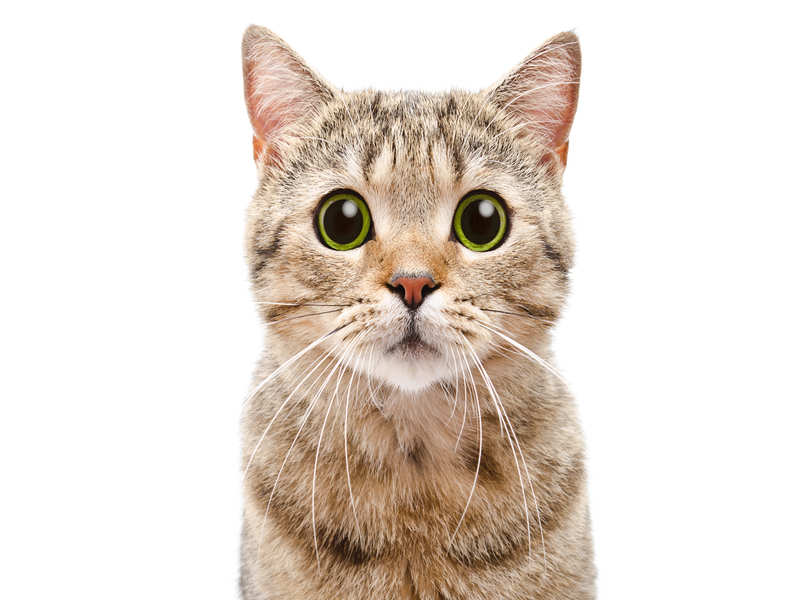
\includegraphics[width=\linewidth]{cat}
        \caption{Figure 1}
    \end{subfigure}
    \hfill
    \begin{minipage}[b]{0.3\textwidth}
	    \begin{subfigure}[b]{\linewidth}
	        \centering
	        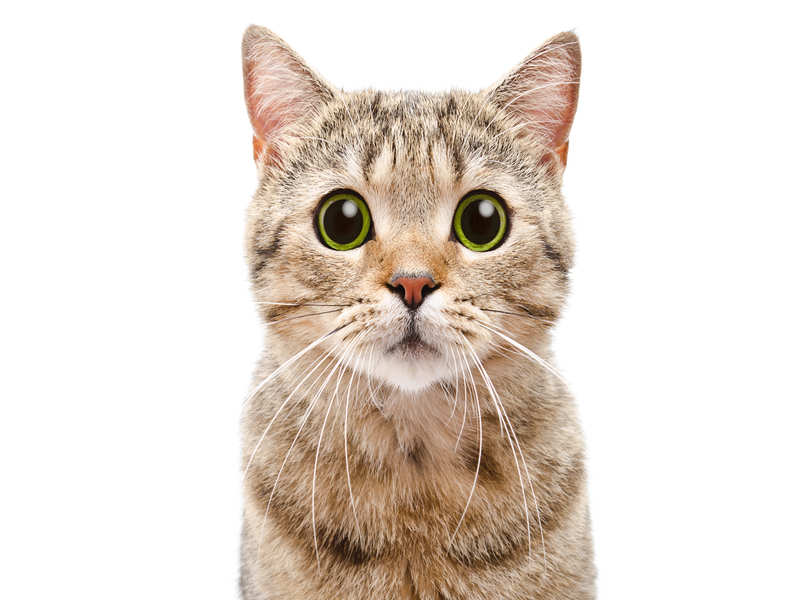
\includegraphics[width=\linewidth]{cat}
	        \caption{Figure 2}
	    \end{subfigure}
	    \\
	    \begin{subfigure}[b]{\linewidth}
	        \centering
	        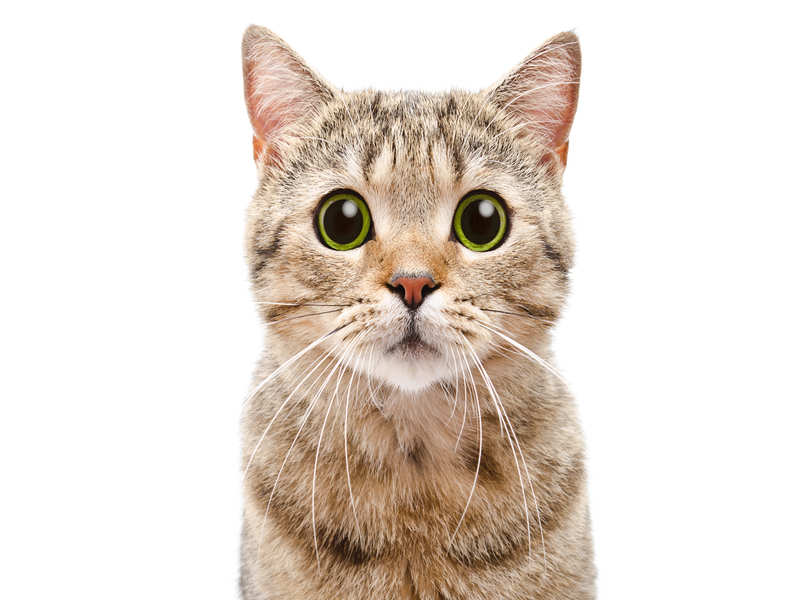
\includegraphics[width=\linewidth]{cat}
	        \caption{Figure 3}
	    \end{subfigure}
	\end{minipage}
    \caption{Subfigures in One Figure (1).}
    \label{fig:subfigures-1}
\end{figure*}

\begin{figure*}[ht!]
    \centering
    \begin{subfigure}[b]{0.67\textwidth}
        \centering
        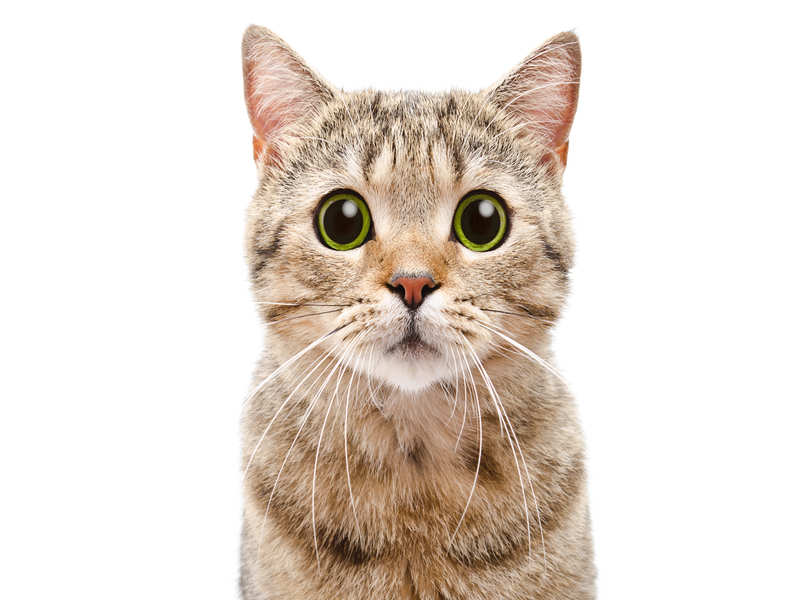
\includegraphics[width=\linewidth]{cat}
        \caption{Figure 1}
    \end{subfigure}
    ~
    \begin{subfigure}[b]{0.67\textwidth}
        \centering
        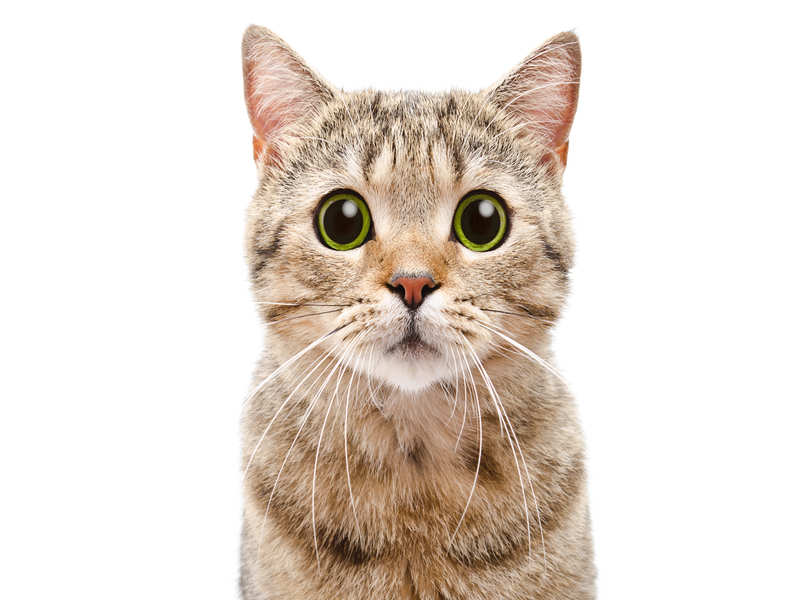
\includegraphics[width=\linewidth]{cat}
        \caption{Figure 2}
    \end{subfigure}
    \caption{Subfigures in One Figure (2).}
    \label{fig:subfigures-2}
\end{figure*}

\section{Landscape Page}

\begin{landscape}
\scriptsize{
\begin{longtable}[]{@{}lllll@{}}
\toprule
Subnet & IPv4 Address / Prefix & IPv4 Address Range & IPv6
Address / Prefix & IPv6 Address Range\tabularnewline
\midrule
\endhead
\texttt{BT-R001} - \texttt{BT001} & \texttt{23.0.0.0/28} &
\texttt{23.0.0.1} - \texttt{23.0.0.14} & \texttt{2001:2300:0:0::/64} &
\texttt{2001:2300:0:0::1} -
\texttt{2001:2300:0:0:ffff:ffff:ffff:fffe}\tabularnewline
\texttt{BT-R002} - \texttt{BT002} & \texttt{23.0.0.16/28} &
\texttt{23.0.0.17} - \texttt{23.0.0.30} & \texttt{2001:2300:0:1::/64} &
\texttt{2001:2300:0:1::1} -
\texttt{2001:2300:0:1:ffff:ffff:ffff:fffe}\tabularnewline
\texttt{BT-R003} - \texttt{BT003} & \texttt{23.0.0.32/28} &
\texttt{23.0.0.33} - \texttt{23.0.0.62} & \texttt{2001:2300:0:2::/64} &
\texttt{2001:2300:0:2::1} -
\texttt{2001:2300:0:2:ffff:ffff:ffff:fffe}\tabularnewline
\texttt{BT-R001} - \texttt{BT-R002} & \texttt{23.0.0.48/30} &
\texttt{23.0.0.49} - \texttt{23.0.0.50} & \texttt{2001:2300:0:3::/64} &
\texttt{2001:2300:0:3::1} -
\texttt{2001:2300:0:3:ffff:ffff:ffff:fffe}\tabularnewline
\texttt{BT-R002} - \texttt{BT-R003} & \texttt{23.0.0.52/30} &
\texttt{23.0.0.53} - \texttt{23.0.0.54} & \texttt{2001:2300:0:4::/64} &
\texttt{2001:2300:0:4::1} -
\texttt{2001:2300:0:4:ffff:ffff:ffff:fffe}\tabularnewline
\texttt{BT-R001} - \texttt{BT-R003} & \texttt{23.0.0.56/30} &
\texttt{23.0.0.57} - \texttt{23.0.0.58} & \texttt{2001:2300:0:5::/64} &
\texttt{2001:2300:0:5::1} -
\texttt{2001:2300:0:5:ffff:ffff:ffff:fffe}\tabularnewline
\texttt{BT-R002} - \texttt{DT} & \texttt{23.0.0.60/30} &
\texttt{23.0.0.61} - \texttt{23.0.0.62} & \texttt{2001:2300:0:6::/64} &
\texttt{2001:2300:0:6::1} -
\texttt{2001:2300:0:6:ffff:ffff:ffff:fffe}\tabularnewline
\texttt{BT-R003} - \texttt{Virgin} & \texttt{56.0.0.60/30} &
\texttt{56.0.0.61} - \texttt{56.0.0.62} & \texttt{2001:5600:0:6::/64} &
\texttt{2001:5600:0:6::1} -
\texttt{2001:5600:0:6:ffff:ffff:ffff:fffe}\tabularnewline
\texttt{BT-R003} - \texttt{Central} & \texttt{100.100.2.0/30} &
\texttt{100.100.2.1} - \texttt{100.100.2.2} & &\tabularnewline
\bottomrule
\caption{Allocation of IPv4 and IPv6 Addresses to Subnets in BT Network.}
\label{tab:ip}
\end{longtable}
}

\scriptsize{
\begin{longtable}[]{@{}lllllll@{}}
\toprule
Connection & Interface 1 & IPv4 Address & IPv6 Address & Interface 2 & IPv4 Address & IPv6
Address \tabularnewline
\midrule
\endhead
\texttt{BT-R001} - \texttt{BT001} & \texttt{BT-R001}:
\texttt{FastEthernet0/1/0} & \texttt{23.0.0.1} &
\texttt{2001:2300:0:0::1} & \texttt{BT001}: \texttt{eth0} &
\texttt{23.0.0.2} & \texttt{2001:2300:0:0::2}\tabularnewline
\texttt{BT-R002} - \texttt{BT002} & \texttt{BT-R002}:
\texttt{FastEthernet0/1/0} -\textgreater{} \texttt{Vlan\ 1} &
\texttt{23.0.0.17} & \texttt{2001:2300:0:1::1} & \texttt{BT002}:
\texttt{eth0} & \texttt{23.0.0.18} &
\texttt{2001:2300:0:1::2}\tabularnewline
\texttt{BT-R003} - \texttt{BT003} & \texttt{BT-R003}:
\texttt{FastEthernet0/1/0} -\textgreater{} \texttt{Vlan\ 2} &
\texttt{23.0.0.33} & \texttt{2001:2300:0:2::1} & \texttt{BT003}:
\texttt{eth0} & \texttt{23.0.0.34} &
\texttt{2001:2300:0:2::2}\tabularnewline
\texttt{BT-R001} - \texttt{BT-R002} & \texttt{BT-R001}:
\texttt{FastEthernet0/0} & \texttt{23.0.0.49} &
\texttt{2001:2300:0:3::1} & \texttt{BT-R002}: \texttt{FastEthernet0/0} &
\texttt{23.0.0.50} & \texttt{2001:2300:0:3::2}\tabularnewline
\texttt{BT-R002} - \texttt{BT-R003} & \texttt{BT-R002}:
\texttt{FastEthernet0/1} & \texttt{23.0.0.53} &
\texttt{2001:2300:0:4::1} & \texttt{BT-R003}: \texttt{FastEthernet0/1} &
\texttt{23.0.0.54} & \texttt{2001:2300:0:4::2}\tabularnewline
\texttt{BT-R001} - \texttt{BT-R003} & \texttt{BT-R001}:
\texttt{FastEthernet0/1} & \texttt{23.0.0.57} &
\texttt{2001:2300:0:5::1} & \texttt{BT-R003}: \texttt{FastEthernet0/0} &
\texttt{23.0.0.58} & \texttt{2001:2300:0:5::2}\tabularnewline
\texttt{BT-R002} - \texttt{DT} & \texttt{BT-R002}:
\texttt{FastEthernet0/1/1} -\textgreater{} \texttt{Vlan\ 3} &
\texttt{23.0.0.61} & \texttt{2001:2300:0:6::1} & \texttt{DT} &
\texttt{23.0.0.62} & \texttt{2001:2300:0:6::2}\tabularnewline
\texttt{BT-R003} - \texttt{Virgin} & \texttt{BT-R003}:
\texttt{FastEthernet0/1/2} -\textgreater{} \texttt{Vlan\ 4} &
\texttt{56.0.0.62} & \texttt{2001:5600:0:6::2} & \texttt{Virgin} &
\texttt{56.0.0.61} & \texttt{2001:5600:0:6::1}\tabularnewline
\texttt{BT-R003} - \texttt{Central} & \texttt{BT-R003}:
\texttt{FastEthernet0/1/1} -\textgreater{} \texttt{Vlan\ 5} &
\texttt{100.100.2.2} & & \texttt{Central} & \texttt{100.100.2.1}
&\tabularnewline
\bottomrule
\caption{Interfaces for Each Physical Connection and Corresponding IPv4 and IPv6 Addresses.}
\label{tab:interfaces}
\end{longtable}
}

\end{landscape}

% \include{Chapter/Requirements}
% \include{Chapter/Design}
% \include{Chapter/Testing}
% \chapter{Conclusions}
\label{chap:discussion}

% In this project we have successfully developed and tested two behaviours for our robot. 
% The first one is Reactive behaviour, which we refer to Braitenberg’s four behaviours, ‘ Love’, ‘Curious’, ‘Aggression’, ‘Fear’. We made our robot able to act four different behaviour regarding to a targeted object, a backpack. The robot itself are able to wonder around the lab and looking for the backpack, after it gather the targeted object in its camera, it will execute the behaviour that we have assigned to it. 
% We have designed a following behaviour to our robot as well, robot will firstly choose a human to follow, analysis that human’s details and then start to follow him in a desire distance, it will turn its direction as well. We also add interrupt function, which means even another person come in through the testing, even fully block the person that robot firstly chosen, robot will still be able to recognize the initial target and still follow that target.

In this coursework, both Reactive Behaviours and Following Behaviours of mobile robot are designed and implemented.
The robot with Reactive Behaviours mimics Braitenberg behaviors, more specifically love, aggression, fear and curiosity.
The robot first wanders around the environment to locate the object of interest (backpack in this case). Once the object is located, a  Braitenberg behavior is performed by the robot.

The robot with Following Behaviours keeps following the designated person on the scene while keeping a safe distance.
The robot first wanders around the environment to locate the person of interest.
Once the designated person is located, the robot moves toward the person while maintaining a safe distance.
In the scenario of possible hijacking by another person, the robot distinguishes between the two persons and only follows the person with the highest similarity score.

Testing procedures are proposed and performed on both tasks. The testing results show that our design and implementation is correct and robust.



% Include a Chapter names References to the table of content
\addcontentsline{toc}{chapter}{References}
% Rename Bibliography to References
\renewcommand\bibname{References}
\bibliography{Bib/tex}

% Include authors publications and appendix section
% \addcontentsline{toc}{chapter}{Publications}
\chapter*{Publications}
\label{chap:Publications}

% Author publication section
% If not using the references per chapter option you need to include the bibliography inline
% This was done by creating a bibtex file containing the publications and including in a separate LaTeX file, using \nocite{*} this includes all bibtex items, generating the .bbl file and then copying and pasting below.

List of authors academic publications

\begingroup
% Remove title and space of header for this chapter
\titleformat{\chapter}[display]
    {\normalfont\huge\bfseries}{\chaptertitlename\ \thechapter}{20pt}{\Huge}
\titlespacing*{\chapter}{0pt}{0pt}{-80pt}
\renewcommand\bibname{}
\begin{thebibliography}{1}

%\bibitem{}

\end{thebibliography}
\endgroup

% To include copies of the publications use the includepdf package and point to .pdf files of papers
% Example
%\includepdf[pages=-, pagecommand=, templatesize={5in}{10in}]{Publications/Pubs/le1_biothreads.pdf}

% Appedix
\appendix

\begingroup

\chapter{Source Code}
\label{app:code}


\section{JPEG CODEC Code in Python}
\label{app:sec:python}

\subsection{Python-MATLAN Interface \texttt{matlab.py}}
\lstinputlisting[caption={Code of Python-MATLAN Interface \texttt{matlab.py}.},captionpos=t,language=Python]{Code/matlab.py}


\endgroup


\end{document}
